%% BioMed_Central_Tex_Template_v1.06
% * <junya009@live.missouristate.edu> 2018-02-22T05:46:56.449Z:
%
% ^.
%%                                      %
%  bmc_article.tex            ver: 1.06 %
%                                       %

%%IMPORTANT: do not delete the first line of this template
%%It must be present to enable the BMC Submission system to
%%recognise this template!!

%%%%%%%%%%%%%%%%%%%%%%%%%%%%%%%%%%%%%%%%%
%%                                     %%
%%  LaTeX template for BioMed Central  %%
%%     journal article submissions     %%
%%                                     %%
%%          <8 June 2012>              %%
%%                                     %%
%%                                     %%
%%%%%%%%%%%%%%%%%%%%%%%%%%%%%%%%%%%%%%%%%


%%%%%%%%%%%%%%%%%%%%%%%%%%%%%%%%%%%%%%%%%%%%%%%%%%%%%%%%%%%%%%%%%%%%%
%%                                                                 %%
%% For instructions on how to fill out this Tex template           %%
%% document please refer to Readme.html and the instructions for   %%
%% authors page on the biomed central website                      %%
%% http://www.biomedcentral.com/info/authors/                      %%
%%                                                                 %%
%% Please do not use \input{...} to include other tex files.       %%
%% Submit your LaTeX manuscript as one .tex document.              %%
%%                                                                 %%
%% All additional figures and files should be attached             %%
%% separately and not embedded in the \TeX\ document itself.       %%
%%                                                                 %%
%% BioMed Central currently use the MikTex distribution of         %%
%% TeX for Windows) of TeX and LaTeX.  This is available from      %%
%% http://www.miktex.org                                           %%
%%                                                                 %%
%%%%%%%%%%%%%%%%%%%%%%%%%%%%%%%%%%%%%%%%%%%%%%%%%%%%%%%%%%%%%%%%%%%%%

%%% additional documentclass options:
%  [doublespacing]
%  [linenumbers]   - put the line numbers on margins

%%% loading packages, author definitions

%\documentclass[twocolumn]{bmcart}% uncomment this for twocolumn layout and comment line below
\documentclass{bmcart}

%%% Load packages
%\usepackage{etoolbox}
\usepackage{amsthm,amsmath}
%\RequirePackage{natbib}
%\RequirePackage[authoryear]{natbib}% uncomment this for author-year bibliography
%\RequirePackage{hyperref}
\usepackage[utf8]{inputenc} %unicode support
%\usepackage[applemac]{inputenc} %applemac support if unicode package fails
%\usepackage[latin1]{inputenc} %UNIX support if unicode package fails
\usepackage{rotating}
\usepackage{subfigure}
\usepackage{makecell}
\usepackage{comment}
\usepackage{amsthm}
\usepackage{amsmath}
\usepackage{amssymb}
\usepackage{graphicx}
\usepackage{threeparttable, tablefootnote}
\usepackage{multirow}
\usepackage{booktabs}
\usepackage{enumerate}
\usepackage{textcomp}
% http://ctan.org/pkg/enumerate
%\usepackage{natbib}
%%%%%%%%%%%%%%%%%%%%%%%%%%%%%%%%%%%%%%%%%%%%%%%%%
%%                                             %%
%%  If you wish to display your graphics for   %%
%%  your own use using includegraphic or       %%
%%  includegraphics, then comment out the      %%
%%  following two lines of code.               %%
%%  NB: These line *must* be included when     %%
%%  submitting to BMC.                         %%
%%  All figure files must be submitted as      %%
%%  separate graphics through the BMC          %%
%%  submission process, not included in the    %%
%%  submitted article.                         %%
%%                                             %%
%%%%%%%%%%%%%%%%%%%%%%%%%%%%%%%%%%%%%%%%%%%%%%%%%


%\def\includegraphic{}
%\def\includegraphics{}



%%% Put your definitions there:
\startlocaldefs
\endlocaldefs


%%% Begin ...
\begin{document}

%%% Start of article front matter
\begin{frontmatter}

\begin{fmbox}
\dochead{Research}

%%%%%%%%%%%%%%%%%%%%%%%%%%%%%%%%%%%%%%%%%%%%%%
%%                                          %%
%% Enter the title of your article here     %%
%%                                          %%
%%%%%%%%%%%%%%%%%%%%%%%%%%%%%%%%%%%%%%%%%%%%%%

\title{Applications of Node-Based Resilience Graph Theoretic Framework to Clustering
Autism Spectrum Disorders Phenotypes}

%%%%%%%%%%%%%%%%%%%%%%%%%%%%%%%%%%%%%%%%%%%%%%
%%                                          %%
%% Enter the authors here                   %%
%%                                          %%
%% Specify information, if available,       %%
%% in the form:                             %%
%%   <key>={<id1>,<id2>}                    %%
%%   <key>=                                 %%
%% Comment or delete the keys which are     %%
%% not used. Repeat \author command as much %%
%% as required.                             %%
%%                                          %%
%%%%%%%%%%%%%%%%%%%%%%%%%%%%%%%%%%%%%%%%%%%%%%

\author[
   addressref={aff1},                   % id's of addresses, e.g. {aff1,aff2}
 %  noteref={n1},                        % id's of article notes, if any
   email={jmatta@siue.edu}   % email address
]{\inits{JM}\fnm{John} \snm{Matta}}
\author[
   addressref={aff2},
   email={Junya009@live.missouristate.edu}
]{\inits{JZ}\fnm{Junya} \snm{Zhao}}
\author[
   addressref={aff1},
   email={gercal@siue.edu}
]{\inits{GE}\fnm{Gunes} \snm{Ercal}}
\author[
   addressref={aff3},
      corref={aff3},                      % id of corresponding address, if any
   email={tayoobafemiajayi@missouristate.edu}
]{\inits{TO}\fnm{Tayo} \snm{Obafemi-Ajayi}}

%%%%%%%%%%%%%%%%%%%%%%%%%%%%%%%%%%%%%%%%%%%%%%
%%                                          %%
%% Enter the authors' addresses here        %%
%%                                          %%
%% Repeat \address commands as much as      %%
%% required.                                %%
%%                                          %%
%%%%%%%%%%%%%%%%%%%%%%%%%%%%%%%%%%%%%%%%%%%%%%

\address[id=aff1]{%                           % unique id
  \orgname{Department of Computer Science, Southern Illinois University Edwardsville}, % university, etc
 % \street{Waterloo Road},                     %
  %\postcode{}                                % post or zip code
  \city{Edwardsville, IL},                              % city
  \cny{USA}                                    % country
}
\address[id=aff2]{%
  \orgname{Department of Computer Science, Missouri State University},
 % \street{D\"{u}sternbrooker Weg 20},
 % \postcode{24105}
  \city{Springfield, MO},
  \cny{USA}
}
\address[id=aff3]{%
  \orgname{Engineering Program, Missouri State University},
 % \street{D\"{u}sternbrooker Weg 20},
 % \postcode{24105}
   \city{Springfield, MO},
  \cny{USA}
}

%%%%%%%%%%%%%%%%%%%%%%%%%%%%%%%%%%%%%%%%%%%%%%
%%                                          %%
%% Enter short notes here                   %%
%%                                          %%
%% Short notes will be after addresses      %%
%% on first page.                           %%
%%                                          %%
%%%%%%%%%%%%%%%%%%%%%%%%%%%%%%%%%%%%%%%%%%%%%%

%\begin{artnotes}
%\note{Sample of title note}     % note to the article
%\note[id=n1]{Equal contributor} % note, connected to author
%\end{artnotes}
\end{fmbox}% comment this for two column layout
%%%%%%%%%%%%%%%%%%%%%%%%%%%%%%%%%%%%%%%%%%%%%%
%%                                          %%
%% The Abstract begins here                 %%
%%                                          %%
%% Please refer to the Instructions for     %%
%% authors on http://www.biomedcentral.com  %%
%% and include the section headings         %%
%% accordingly for your article type.       %%
%%                                          %%
%%%%%%%%%%%%%%%%%%%%%%%%%%%%%%%%%%%%%%%%%%%%%%
\begin{abstractbox}
\begin{abstract}% abstract
With the growing ubiquity of data in network form, clustering in the context of a network, represented as a graph, has become increasingly important. Clustering is a very useful data exploratory machine learning tool that allows us to make better sense of heterogeneous data by grouping data with similar attributes based on some criteria. This paper investigates the application of a novel graph theoretic clustering method, Node-Based Resilience clustering (NBR-Clust), to address the heterogeneity of Autism Spectrum Disorder (ASD) and identify meaningful subgroups. 
The hypothesis is that analysis of these subgroups would reveal relevant biomarkers
that would provide a better understanding of ASD phenotypic heterogeneity useful for further ASD
studies. We address appropriate graph constructions suited for representing the ASD phenotype
data. The sample population is drawn from a very large rigorous dataset: Simons Simplex
Collection (SSC). Analysis of the results performed using
graph quality measures, internal cluster validation measures,  and clinical analysis outcome demonstrate the potential usefulness of resilience measure clustering for biomedical datasets. We also conduct feature extraction analysis to characterize relevant biomarkers that delineate the resulting subgroups. 
The optimal results obtained favored predominantly a 5-cluster configuration.


\end{abstract}

%%%%%%%%%%%%%%%%%%%%%%%%%%%%%%%%%%%%%%%%%%%%%%
%%                                          %%
%% The keywords begin here                  %%
%%                                          %%
%% Put each keyword in separate \kwd{}.     %%
%%                                          %%
%%%%%%%%%%%%%%%%%%%%%%%%%%%%%%%%%%%%%%%%%%%%%%

\begin{keyword}
\kwd{graph theory}
\kwd{clustering} 
\kwd{autism spectrum disorders}
\kwd{resilience measures}
\end{keyword}

% MSC classifications codes, if any
%\begin{keyword}[class=AMS]
%\kwd[Primary ]{}
%\kwd{}
%\kwd[; secondary ]{}
%\end{keyword}

\end{abstractbox}
%
%\end{fmbox}% uncomment this for twcolumn layout

\end{frontmatter}

%%%%%%%%%%%%%%%%%%%%%%%%%%%%%%%%%%%%%%%%%%%%%%
%%                                          %%
%% The Main Body begins here                %%
%%                                          %%
%% Please refer to the instructions for     %%
%% authors on:                              %%
%% http://www.biomedcentral.com/info/authors%%
%% and include the section headings         %%
%% accordingly for your article type.       %%
%%                                          %%
%% See the Results and Discussion section   %%
%% for details on how to create sub-sections%%
%%                                          %%
%% use \cite{...} to cite references        %%
%%  \cite{koon} and                         %%
%%  \cite{oreg,khar,zvai,xjon,schn,pond}    %%
%%  \nocite{smith,marg,hunn,advi,koha,mouse}%%
%%                                          %%
%%%%%%%%%%%%%%%%%%%%%%%%%%%%%%%%%%%%%%%%%%%%%%

%%%%%%%%%%%%%%%%%%%%%%%%% start of article main body
% <put your article body there>

%%%%%%%%%%%%%%%%
%% Background %%
%%

\section*{Introduction}
\label{sec:intro}

Clustering comprises a prolific research area for data exploration and knowledge discovery applications with a great variety of approaches. %\cite{ClusteringBook}. 
With the growing ubiquity of data in network form, clustering in the context of a network represented as a graph has become increasingly important.
In graph theory contexts, clustering involves finding a k-partitioning of the vertices of a graph. 
The concepts and properties of graph theory make it very convenient to describe clustering problems by means of graphs \cite{xu2009clustering}.  Nodes $V = \{v_i, i = 1 , ... , N\}$ of a weighted graph $G$ correspond to $N$ data points in the pattern space, and edges $E = \{e_{ij}, i,j \in V, i \neq j\}$ reflect the proximities between each pair of data points.
%Optimal partitioning configurations generally have the property that edges are denser within a cluster and less dense between clusters.  There may be additional constraints on clusters, such as on the relative size of each group % \cite{ShiMalik}, \cite{alpert1999spectral}. 
Use of graph theoretic clustering techniques is not restricted to cases where the data is inherently graph-based. They have also been shown to be effective on other types of data by transforming the data to a graph form using an appropriate graph representation \cite{alpert1999spectral}. Brugere et al.~\cite{Brugere2018} provide an in depth overview regarding creating networks from data as well as examples of network structure inference in diverse fields such as computational biology, neuroscience, epidemiology, ecology, and mobile device technology.

There are many benefits to converting data to a network representation as networks are an excellent way of representing complex relationships. The following benefits are highlighted and discussed in details in Ref.~\cite{Brugere2018}. Networks aid in uncovering the higher-order structure emerging from dyadic relationships. They are also useful in exploring the heterogeneity that exists among individual entities. 
%Many different means exist for interpreting networks, including simple measures such as density, degree distribution, clustering coefficient and centralities as well as more complex measures such as robustness and routing efficiency. 
Diverse measures can be applied in interpreting and/or evaluating network representations such as density, degree distribution, clustering coefficient, centralities, etc.  
Networks are interpretable models for further analysis and hypothesis generation. Many useful tools also exist for network analysis that can be used across domains. Thus, networks provide a common language through which biological researchers can communicate with computer scientists. Graph based methods aid ease of visualization of analysis, a natural co-occurrence of network representation. Given a dataset, the main challenge usually lies in determining which particular network will be the most useful representation to provide  meaningful inference.


There are various successful examples of the use of graphs in analyzing biological and health-related data. 
Pan et al.~\cite{ETV5Tumor} converted gene expression data to an appropriate graph representation and computed \textit{betweenness centrality} (a graph-theoretic measure) to find important regulator genes in tumors. 
Their study is a useful motivation for the current work, which also uses betweenness centrality in a heuristic to find important data points. 
%Motivated by the work of Lanke et al. \cite{ETV5Tumor}, in this current work, we also apply betweenness centrality in a heuristic to find important data points. 
%Gene interaction networks are good candidates for graph representation \cite{Brugere2018}. 
%In \cite{monaco2018complex}, gene networks are analyzed for linkage to schizophrenia.
%Lanke et al. \cite{LankeAlzheimers} analyzed gene co-expression networks and protein–protein interaction networks to identify network-level changes in the brain that mark the transition from young to Alzheimer's.
Dale et al. \cite{grapevine} employed graph clustering techniques to gene expression data to identify genes potentially related to powdery mildew disease resistance in grapevines.  
Alves et al. \cite{alves2018graph} applied graph clustering and graph theoretic measures (degree distribution, average clustering coefficient, and average short path length) to evaluate the effects of an antibody on chick embryos. 
The specific application of classification of human traits and diseases in patient networks using graph analysis is conducted for a variety of medical applications including pathological narcissism in \cite{DIPIERRO2018}, dark personality traits in \cite{MARCUS201856}, post-traumatic stress disorder in \cite{akiki2018default}, and inflammatory bowel diseases in \cite{yasser}. 
%Due to the focus of edge cuts as splitting a component into two parts, such edge-based approaches must either be used hierarchically or iteratively with either an external stopping condition or with the desired number of clusters as input.

%Popular graph theoretic clustering algorithms include Girvan-Newman \cite{GirvanNewman} and variations of spectral clustering methods \cite{nascimento2011spectral}.  These methods may be viewed as solving an edge-based resilience problem on a graph and outputting the components resulting from the removal of the critical attack set of edges as the set of clusters. 


%NBR-Clust has been applied to biological datasets \cite{Grapevine,DREAM} as well as to the ASD phenotype based datasets used in this work\cite{BICOB} with promising preliminary results. 

This paper investigates the application of graph theoretic clustering on analysis of clinical data relating to Autism Spectrum Disorder (ASD) phenotypes.
Clinical data, such as in ASD, is commonly characterized by significant heterogeneity, high dimensionality, complexity in structure and mixture of variables, disparate data sources, and missing data. There is a critical need to identify and validate more homogeneous subgroups as well as learn the distinct features (biomarkers) associated with the subgroups. This work significantly extends preliminary results presented in \cite{BICOB} on clustering ASD phenotype data using our \emph{node-based resilience} clustering framework (NBR-Clust) \cite{ICDM,FLAIRS}.
%on application of the node-based graph theoretic clustering algorithms to address the heterogeneity of Autism Spectrum Disorder (ASD) clinical data and identify meaningful subgroups.}  
NBR-Clust is unique in its focus on critical attack sets of \emph{nodes} $S \subset V$ whose removal disconnects the network into multiple components that form the basis of resultant clusters.  Due to natural properties of sparse node-cuts, the NBR-Clust approach is useful not only for traditional clustering scenarios where the number of clusters may be unknown \textit{a priori}, but also for clustering in the presence of outliers or noise, and/or overlapping nodes \cite{ICDM,FLAIRS}. 
In \cite{ICDM}, we generalized the usefulness of node-based resilience measures for clustering, particularly when the number of clusters is not known \textit{a priori}. We conducted an in-depth comparative analysis using existing known resilience measures such as integrity, toughness, tenacity, and scattering number as well as a parametrized version of vertex attack tolerance (VAT). The results obtained demonstrated the effectiveness of VAT and integrity over the other methods in clustering the datasets with high accuracy.  Additionally, integrity was likely to cluster datasets in one step, and tenacity was useful for giving an upper bound to cluster number determination. 

In this work, we conduct a systematic exploration of application of NBR measures to delineate heterogeneous ASD data into more meaningful subgroups using a sample population drawn from the Simons Simplex Collection \cite{fischbach2010simons}. We investigate three NBR measures (VAT, Integrity and Tenacity) along with multiple graph constructions to determine appropriate representations for the ASD phenotype data. We also employ feature extraction techniques to determine a potential set of ASD phenotype biomarkers that discriminate the resulting subgroups. A varied set of statistical methods is applied to validate and interpret the clinical significance of the results.

%Thus, the objective is to apply graph theoretical clustering models to aid a biomedical problem: categorizing ASD patients into more meaningful homogeneous groups. The goal is that the resulting clusters would provide a better understanding of ASD phenotypic heterogeneity and delineate subgroups useful for further ASD studies. We are also interested in investigating the appropriate   We compare the performance of our methods to spectral clustering using varied internal cluster validation indices \cite{liu2010understanding}.



\section*{Autism Spectrum Disorders}
\label{sec:asd}

ASDs are childhood neurodevelopmental disorders diagnosed on the basis of behavioral assessments of social, communicative, and repetitive symptoms \cite{DSM}. Although ASD is behaviorally distinctive and reliably identified by experienced clinicians, it is clinically and genetically extremely heterogeneous \cite{miles2011autism}. Children with ASD exhibit a wide diversity in type, number, and severity of social deficits, behaviors, and communicative and cognitive difficulties, which are assumed to reflect multiple etiologic origins \cite{eaves1994subtypes}. Given the increase in ASD prevalence \cite{autism2014prevalence} and the corresponding increasing associated economic burden \cite{lavelle2014economic}, there is a need for automated approaches to detect more homogeneous subgroups of patients, and more importantly for biomarkers (biologically based phenotypes) to inform tailored intervention and improved outcomes. Biomarkers are useful to index diagnostic status or risk, demonstrate engagement of specific biological systems, and provide more rapid assessment of change than traditional measures based on clinical observation and caregiver report \cite{mcpartland2016considerations}. 
%The overall goal is to determine a robust set of phenotype biomarkers that might sort out the etiologic heterogeneity associated with ASD. 
In the unsupervised learning context, biomarkers can be regarded as significant features that characterize a subgroup (or cluster). Thus, the problem of inferring meaningful biomarkers translates to unsupervised learning of discriminant features. 
A better understanding of heterogeneity in autism itself, based on scientifically rigorous approaches centered on systematic evaluation of the clinical and research utility of the phenotypic and genotypic markers \cite{georgiades2013importance}, would generate useful information for the study of etiology, diagnosis, treatment and prognosis of the disorder. 


There have been varied cluster analysis approaches on ASD phenotype/clinical data over the past two decades. Prior to DSM-5 \cite{DSM}, some of these approaches \cite{stevens2000subgroups,ingram2008defining,cuccaro2012exploring} focused on exploring empirical subgroups that aligned with pre-defined subgroups (such as ASD DSM-IV subtypes) or illuminated some knowledge on etiologically distinct subgroups i.e. which behavioral and physical phenotypes will most likely subdivide ASD.  
Since the introduction of the DSM-5, emphasis is placed on the spectrum of autism i.e. on a severity gradient under the diagnostic umbrella of Autism Spectrum Disorder. According to Georgiades et al. \cite{georgiades2013importance}, the task of categorizing the clinical heterogeneity in children with autism is still of critical importance, regardless of how the DSM changes its definition. Hence, there have been even more studies \cite{georgiades2013investigating,ousley2014autism,veatch2014genetically,obafemi2015sorting,al2016ensemble,obafemi2018asd} that attempt to better classify the ASD heterogeneity under DSM-5 using a varied set of ASD phenotype data.
Some ASD studies \cite{chaste2015genome} suggest that attempts to stratify children based on phenotype will not increase the power of ASD genetic discovery studies. This is possibly true when the methods are limited by a very restricted set of phenotyping variables (diagnosis, IQ, age at first words, ASD severity, insistence sameness, and symptom profiles) and do not account for possible outliers in the dataset. Spencer et al. \cite{spencer2018heritable} demonstrated that ASD phenotype subgroups could aid discovery of novel ASD genes.
It is important to employ clustering methods that simultaneously identify and remove possible outliers that could be skewing the results and add pertinent and relevant phenotype ingredients that may uncover meaningful subtypes. Ultimately, the validity of any subgrouping paradigm depends on whether the ASD subgroups actually uncover/expose some biologic or genetic variation, which can be used to predict prognosis, recurrence risks or treatment responses. Hence, in this work, we also apply rigorous statistical analysis to validate the significance of the results as well as guide the optimal clustering configuration selection. 

\section*{Clustering Framework}
\label{sec:nbr}

\subsection*{NBR-Clust Algorithm}

Node-based resilience measures compute a critical attack set of nodes $S \subset V$ whose removal disconnects the network with relative severity.  
Given a node-based resilience measure, NBR-Clust conducts robust clustering by using the set of components that result from the removal of the computed critical attack set as a basis for the set of clusters.  
%In addition to such applicability in noisy or overlapping scenarios, 
%NBR-Clust is useful in cluster number determination in a one-shot non-hierarchical context.
%Although NBR-Clust may take \emph{any} node-based resilience measure as a functional input parameter,
We explore the following three node-based resilience measures in this work: vertex attack tolerance (VAT), integrity, and tenacity.

The VAT of an undirected, connected graph G = (V, E) is denoted $\tau(G)$ and defined as \cite{spectralVAT}, \cite{matta2017vertex}
\begin{equation}
\tau(G) = \min_{S \subset V, S \neq \emptyset} \left\{\frac{|S|}{|V-S-C_{max}(V-S)|+1 } \right\} 
\end{equation}

where $S$ is an attack set and $C_{max}(V-S)$ is the largest connected component in $V-S$. 

%where $C_{max}(V - S)$ is the largest connected component in $V - S$.

Normalized integrity \cite{Barefoot1987} is defined as

\begin{equation}
I(G) = \min_{S \subset V} \left\{ \frac{|S|  + C_{max}(V-S)}{|V|} \right\}.
\end{equation}

Tenacity \cite{Cozzens1995} is defined as \begin{equation}
T(G) = \min_{S \subset V}\left\{\frac{|S|+C_{max}(V-S)}{\omega (V-S)}\right\},
\end{equation} 

where $\omega (V-S)$ is the number of connected components in $V-S$.  



%As previously mentioned, the critical attack set may be used to help determine outlier or overlap data points when relevant.  Only when all nodes of the critical attack set are reassigned to base clusters does a traditional complete clustering result.
Traditional clustering usually ensures assignment of all nodes to a specific cluster.
In complex datasets, some nodes could be outliers (nodes that don't really belong to a specific cluster) or overlapping nodes (i.e. nodes that could be assigned to more than one cluster). In these scenarios, the critical attack set may be used to determine outliers or overlap data points\cite{ICDM,FLAIRS}. 
%\textbf{The critical attack set could be reassigned to the appropriate cluster or utilized to compute either \emph{noise} or \emph{overlap} when applicable, as both have been empirically evidenced to be highly correlated to the critical attack set\cite{ICDM,FLAIRS}.}
In this work, we consider both the traditional complete clustering scenario where all critical attack nodes are reassigned to cluster-components, as well as the non-traditional situation where the critical attack set is removed from the base clusters (i.e. without node reassignment). Given that we are clustering phenotype data that could involve some errors from the data collection process, outliers would imply potential erroneous data points. Removal of these outliers may result in better defined clusters. 
Overlap nodes could also be a pertinent feature, like in biological networks when proteins are classified to different clusters to reflect their multiple functions. However, the concept of overlap nodes is not clearly defined for medical data. We plan to explore this concept further in future work.

%We analyze the usefulness of the latter situation in discovering a more refined set of phenotype biomarkers.


The NBR-Clust algorithm consists of four main phases: 
\begin{enumerate}[i)]
\item Transform point data into a graph G;
\item Approximate resilience measure of graph,  R(G), with acceptable accuracy, and return the candidate attack set S whose removal results in some number of candidate groupings (components C);
\item Perform a node-assignment strategy that assigns each node of S to a component C from step ii;
\item If more clusters are desired, choose the component with the lowest resilience measure and divide it into additional components using steps ii and iii. If fewer clusters are desired, join components with the greatest number of adjacent edges. The dividing and combining can continue until a desired number of clusters is obtained.
\end{enumerate}   
 
The VAT-Clust, Integrity-Clust, and Tenacity-Clust algorithms (\cite{FLAIRS}, \cite{ICDM}) utilize a heuristic known as Greedy-betweenness centrality (Greedy-BC). 
%Betweenness centrality is a graph-theoretic measure based on shortest paths. 
The \textit{betweenness centrality} of a node is the ratio of shortest paths that include that node to the total number of shortest paths. High betweenness centrality is a measure of the importance of a node, as it implies that the node is more likely to be part of a path used when traversing the graph.
The Greedy-BC heuristic estimates candidate attack sets by repeatedly taking the highest betweenness node, removing it from the network, taking the next highest betweenness node, removing it from the network, etc. Matta~\cite{matta2017comparison,matta2017vertex} demonstrated that Greedy-BC approximates VAT, integrity and tenacity with acceptable accuracy. We implemented the NBR-Clust framework using weighted betweenness centrality computations \cite{brandes2001faster}. 

%In this work, we focus on applying VAT-Clust, Integrity-Clust, and Tenacity-Clust, and observing results while varying the desired number of clusters, $k$. In previous work, we have observed that VAT tended to produce relatively small attack sets, which led fewer clusters; however accuracy was high.  Integrity also produced highly accurate clusterings, and was useful for determining a natural number of clusters when it was not known \textit{a priori}. Tenacity produced the largest attacks sets, and correspondingly the largest number of clusters.  Tenacity was useful particu[larly for providing an upper bound on natural number of clusters for a given dataset. 

In the NBR-Clust method, if there is a desired number of clusters $k$ for the output clustering configuration, a regrouping or hierarchical \cite{FLAIRS} algorithm can be applied to attain this. 
None of the three clustering algorithms are guaranteed to output an exact $k$ number of clusters.   
When more clusters are produced than desired, we regroup clusters by finding the pair of current components C1 and C2 that maximizes the normalized cut quantity: E(C1,C2)/(C1*C2), where E(C1,C2) is the number of edges between C1 and C2 and C1*C2 is the product of the number of nodes in C1 and the number of nodes in C2.  
%This method of regrouping tends to cause smaller clusters to be combined into larger clusters. 
C1 and C2 are combined into one cluster. Regrouping of clusters is repeated until the desired number of clusters is obtained. 
If the algorithm outputs fewer clusters than desired, then the hierarchical approach \cite{FLAIRS} is applied to split the clusters till the specified number of clusters is achieved. 

\subsection*{Data Preprocessing}
Given that the sample was drawn from a rigorous data collection (Simons Simplex Collection \cite{fischbach2010simons}, it contained very few missing values, approximately 0.1\% missing values.  Majority of the missing values were localized in two features, out of a total of 36 features. To impute missing values for these two attributes we used a standard regression, computed in Matlab, on the remaining 34 attributes to determine likely values. For other features that had very few missing values ($0.002\%$), the mean of the remaining values for the specific feature was used. 

Feature selection is commonly used for selecting a small subset of features for building a learning model with good generalization performance \cite{guyon2003introduction}. Usually, the task of a feature selection algorithm is to prune the feature space by eliminating as many irrelevant and redundant features as possible and thus reducing the dimensionality of the dataset. In the dataset used, the number of features is relatively small compared to the number of examples.
%The purpose of unsupervised feature selection is to reduce the redundancy in the feature list. 
We apply the correlation filter algorithm introduced in  \cite{obafemi2017unified} to exclude highly correlated features from the subsequent analysis. The filter algorithm automatically identifies and filters highly correlated features using pairwise Pearson correlation function based on a user defined threshold value. In this work, we investigate the effect of applying the correlation filter prior to clustering vs. simply using the entire set of features. 

\subsection*{Graph Representations}

To apply the NBR-Clust framework on our dataset, we first convert the data into a k-nearest neighbor (kNN) graph $G$. In a kNN graph $G_k$, vertices $u$ and $v$ have an edge between them if $v$ is amongst the $k$ closest vertices to $u$ with respect to the distance metric considered.  While any distance metric may be used to determine nearness of neighbors, we use the $n$-dimensional Euclidean distance following normalization of the feature space, where $n$ is the number of features considered.
%Here a table is created by calculating the Euclidean distance $d(p,q)$ between each pair of data points $p, q$, in $n$-dimensional space, where $n$ is the number of features considered.
%such that \[d(p,q) = \sqrt[]{\sum_{i=1}^n (q_i - p_i)^2}.\]  For each node, the $k$ points with the nearest distances are connected to it.

In both \cite{ICDM} and \cite{cukierski2008using} evidence is presented in favor of minimal connectivity (min-conn) parameter $k$ in the construction of kNN graph $G_k$. 
%namely $k$ such that $G$ is connected but disconnected below $k$.
Min-conn $k$ implies choosing the minimal $k$ such that $\: \forall \;k' \ge k \; \forall_{(u, v \in V)}   \; \exists \text{ \textit{u-v} path in } G_{k'}$.
Additional information may be revealed at different levels of connectivity. 
A graph where parameter $k$ is above connectivity contains more information in the form of additional edges. If nodes that should be clustered together are near to each other, edges are more likely to be added within potential clusters than between them. This will make it easier to identify clusters, and may give better clustering results than graphs where $k$ is at minimum connectivity. The cost of using additional information is increased time and complexity.

We consider three different connectivity settings for $k$ in the kNN graph construction: min-conn, min-conn+1, and min-conn+2.  
%Other parametric settings of the graph construction considered involve different normalizations of the data as well as using a correlation filtered versus unfiltered set of features.  
%%%%bring this up in discussion of results
%In confirmation of previous work in favor of minimally connected kNN graphs \cite{cukierski2008using}, we have found that the min-conn setting is the least sensitive to changes in the other parameters while min-conn+2 was most sensitive to normalization and filter algorithm.}

%Given that the minimum connectivity obtained on the actual data in this work was at $k$=2, we could not examine graphs at below minimum connectivity in contrast to preliminary results presented in \cite{BICOB}.}

%The first step of clustering involves transforming point data into graphs.  We transformed our data into kNN graphs.  In a kNN graph, each node is connected to its k nearest neighbors.  In such graphs there is a minimum value for k, as a function of the data distribution, such that graph connectivity is ensured at and above that value but not below it.  In previous work \cite{ICDM, cukierski2008using}, we and others have observed that the minimum connectivity kNN threshold tended to yield both good accuracy and efficiency of clustering.  


%For example, where k is below connectivity, some of the clustering is already done, as the graph initially has more than one component. In this case, hierarchical clustering proceeds by dividing the component with the lowest resilience measurement. 
%  We tested our clustering methodologies on graphs where $k$ = 2, 3 and 4.  


\subsection*{Determining Optimal Clustering Configuration}

We applied a holistic approach in determining the most optimal set of results per resilience measure (VAT, Integrity, and Tenacity) using three main criteria: internal cluster validation indices (ICVIs), graph quality measures, and distribution of resulting clusters.
Clustering configurations that resulted in clusters with very few nodes (i.e. less than 10) were discarded, given that we had a total of 2680 nodes to cluster. Highly un-skewed clustering configurations tend to bias the cluster validation indices.

An internal cluster validation index determines the optimal clustering solution most appropriate for the input dataset based on two measurement criteria: Compactness and Separateness \cite{kovacs2005cluster}. Compactness measures how close the members of each cluster are to each other. Separateness measures how separated the clusters are from each other. The optimal cluster configuration should yield clusters that are compact and well separated. We explored the application of nine commonly used ICVIs \cite{liu2010understanding,liu2013understanding,aggarwal2013data} (Silhouette index (SI), Davies-Bouldin (DB) index, Dunn's index, Xie-Beni index (XB), Calinski-Harabasz (CH) index, I index (I),  SD validity index (SD), S\_Dbw validity index (S\_Dbw), and Clustering Validation index based on Nearest Neighbors (CVNN)) on the clustering results to measure the goodness of the clusters. The metrics are described fully in \cite{liu2010understanding, liu2013understanding} and were implemented following their guidelines. 
We applied a large number of ICVIs to attain a more robust decision, given multiple studies \cite{brun2007model,vendramin2010relative,arbelaitz2013extensive,liu2013understanding} that demonstrate the diversity in range of results chosen by different indices.
The optimal number of clusters is determined based on the majority vote of the validation indices along with the graph validation measures. A summary of these internal validation metrics utilized in this work for selecting the optimal clustering configuration is presented in Table \ref{tab:indices}. The notations and definitions employed are similar to those presented in \cite{liu2013understanding}.

Since the clustering is done on graph representations of the data, we also utilized specific graph quality measures to evaluate the quality of the resulting graphs: modularity \cite{newman2006modularity} and conductance \cite{CondSparse}. 
\begin{enumerate}
\item \textbf{Modularity}: This quantifies the strength of \textit{modules} (analogous to clusters) created when clustering a graph. A graph with high modularity has more than expected edges internal to its modules, and fewer than expected edges between modules.  We applied modularity to evaluate the ``clusterability" of a graph based on a minimal threshold of 0.6.
\item \textbf{Conductance}: The conductance of a cluster is the fraction of all edges in the graph that point outside the cluster \cite{comscore-icdm12}.  A low conductance implies a ``better'' cluster, because a higher proportion of a graph's edges are internal to that cluster. For our experiments, clustering configurations were acceptable conductance-wise if they had a conductance value of 0.07 or less. 

\end{enumerate}


\begin{comment}
\begin{table}[ht!]
\caption{Summary of internal cluster validation used to determine optimal clustering configuration}
\label{tab:indices}
  \centering
%  \begin{tabular}{llc}
\begin{tabular}{llc}
        \hline
\textbf{Validation Metric }& \textbf{Mathematical Description} & \textbf{Optimal Value}  \\
\hline
Silhouette index (SI)  &	$\frac{1}{k}\sum_{i}^{}\bigg\{\frac{1}{n_i}\sum_{x \in C_i}^{}\frac{b(x)-a(x)}{\max_{x}[b(x),a(x)]}\bigg\}$	& Max \\
Calinski-Harabasz index (CH)  &	$\frac{\sum_{i}^{}n_id^2(c_i,c)/(k-1)}{\sum_{i}^{}\sum_{x \in C_i}^{}d^2(x,c_i)/(N-k)}$  &	Max\\
Davies-Bouldin index (DB) & $\frac{1}{k}\sum_{i}\max_{j, j \neq i} \bigg[ \frac{\frac{1}{n_i}\sum_{x \in C_i}d(x,c_i) + \frac{1}{n_j}\sum_{x \in C_j}d(x, c_j)}{d(c_i,c_j)}\bigg]$ &	Min\\
Dunn’s index  &	$\min_{i}\bigg[\min_{j}\frac{\min_{x \in C_i , y \in C_j}d(x,y)}{\max_{k}\max_{x,y \in C_k}d(x,y)}\bigg]$ &	Max\\
Xie-Beni index (XB)  & $\frac{\sum_{i}\sum_{x \in C_i}d^2(x,c_i)} { N  \min_{i,j \neq i}d^2(c_i,c_j)}$ &	Min\\

%\begin{minipage}[t]{0.8\columnwidth}%
SD validity Index (SD) &\makecell{ $Scat(NC) + Dens_bw(NC) $ where \[Scat(NC) = \frac{1}{NC}\sum_{i}||\sigma(C_i)|| / ||\sigma(D)||\] \[Dis(NC) = \frac{\max_{i,j}d(c_i,c_j)}{\min_{i,j}d(c_i,c_j)}\sum_{i}\Big[\sum_{j}d(c_i,c_j)\Big]^{-1}\]} & Min\\
%\end{minipage}

S\_Dbw validity Index (SD) & & Min \\
$I$ index  & $\bigg[\frac{\sum_{x \in D}d(x,c)}{NC \sum_{i}\sum_{x \in C_i}d(x,c_i)}\max_{i,j}d(c_i,c_j)\bigg]^p$ & Max\\
CVNN index  & $ \frac{Sep(NC,k)}{\max\limits_{NC}SEP(NC,k)}  + \frac{Com(NC)}{\max\limits_{NC}Com(NC)} $
where 
\[Com(NC) = \sum_{i}\Big[\frac{2}{n_i(n_i-1)}\sum\limits_{x,y \in C_i}d(x,y)\Big]\]
\[Sep(NC,k) = \max_i(\frac{1}{n_i}\sum_{j}^{n_i}\frac{q_j}{k})\] &  Min\\
\hline
\end{tabular}
\begin{tablenotes}\footnotesize
\item $D$ denote the data set; $N$: number of objects in $D$; $C$: center of $D$; 
\item $k$: number of clusters; $C_i$: the i–th cluster; $n_i$: number of objects in $C_i$; 
\item $c_i$: center of $C_i$; $d(x,y)$: distance between $x$ and $y$.
\end{tablenotes}
\end{table}
\end{comment}

%--------------------------
\begin{table}[ht!]
\caption{Summary of internal cluster validation used to determine optimal clustering configuration}
\label{tab:indices}
  \centering
%  \begin{tabular}{llc}
\begin{tabular}{lll}
        \hline
\textbf{\makecell[l]{\rule{0pt}{3ex}Validation\\Metric} }& \textbf{Mathematical Description} & \textbf{\makecell[l]{Optimal\\Value}}  \\
\hline%--------------
\rule{0pt}{5ex}\makecell[l]{Silhouette\\index (SI)}  &	
\begin{tabular}{l}
\rule{0pt}{5ex}$\frac{1}{k}\sum_{i}^{}\bigg\{\frac{1}{n_i}\sum_{x \in C_i}^{}\frac{b(x)-a(x)}{\max_{x}[b(x),a(x)]}\bigg\}$	where \\
\rule{0pt}{5ex}$a(x) = \frac{1}{n_i - 1} \sum_{y \in c_i, y \neq x} d(x,y)$ and\\ 
\rule{0pt}{5ex}$b(x) = min_{j, j\neq i}\bigg[ \frac{1}{n_j} \sum_{y \in C_j} d(x,y) \bigg]$ \\
\end{tabular}
& Max \\ 
\noalign{\vskip 2mm}  
\hline
\rule{0pt}{5ex}\makecell[l]{Calinski-\\Harabasz\\index (CH)}  &	$\frac{\sum_{i}^{}n_id^2(c_i,c)/(k-1)}{\sum_{i}^{}\sum_{x \in C_i}^{}d^2(x,c_i)/(N-k)}$  &	Max\\
\noalign{\vskip 2mm}
\hline
\rule{0pt}{5ex}\makecell[l]{Davies-\\Bouldin\\index (DB)} & $\frac{1}{k}\sum_{i}\max_{j, j \neq i} \bigg[ \frac{\frac{1}{n_i}\sum_{x \in C_i}d(x,c_i) + \frac{1}{n_j}\sum_{x \in C_j}d(x, c_j)}{d(c_i,c_j)}\bigg]$ &	Min\\
\noalign{\vskip 2mm}
\hline
\rule{0pt}{5ex}Dunn’s index  &	$\min_{i}\bigg[\min_{j}\frac{\min_{x \in C_i , y \in C_j}d(x,y)}{\max_{k} \{\max_{x,y \in C_k} d(x,y) \}}\bigg]$ &	Max\\
\noalign{\vskip 2mm}
\hline
\rule{0pt}{5ex}\makecell[l]{Xie-Beni\\index (XB)}  & $\frac{\sum_{i}\sum_{x \in C_i}d^2(x,c_i)} { N  \min_{i,j \neq i}d^2(c_i,c_j)}$ &	Min\\
\noalign{\vskip 2mm}
\hline

\makecell[l]{SD validity\\index (SD)} 
&\begin{tabular}{l}%{p{6cm}}
\rule{0pt}{4ex}%
$Dis(k_{max})Scat(k) + Dis(k)$ where \\
\rule{0pt}{4ex}$Scat(k) = \frac{1}{k}\sum_{i}||\sigma(C_i)|| / ||\sigma(D)||$ and\\
\rule{0pt}{4ex}$Dis(k) = \frac{\max_{i,j}d(c_i,c_j)}{\min_{i,j}d(c_i,c_j)}\sum_{i}\Big[\sum_{j}d(c_i,c_j)\Big]^{-1}$%\] 

\end{tabular}
& 
Min\\
\noalign{\vskip 2mm}
\hline
\rule{0pt}{5ex}\makecell[l]{S\_Dbw\\ validity\\Index\\(SD\_Dbw)} &
\begin{tabular}{l}
\rule{0pt}{5ex}$Scat(k) + Dens\_bw(k)$ where \\
$Dens\_bw(k) = \frac{1}{k(k-1)} \sum\limits_i \bigg[ \sum\limits_{j, j \neq i} \frac{\sum\limits_{x \in C_i \cup C_j}f(x, u_{ij})}{max \big\{ \sum\limits_{x \in C_i}f(x,c_i),\sum\limits_{x \in C_j}f(x,c_j) \big\}} \bigg]$\\
\end{tabular}
& Min \\
\noalign{\vskip 2mm}
\hline
\rule{0pt}{5ex}$I$ index  & $\bigg[\frac{\sum_{x \in D}d(x,c)}{k \sum_{i}\sum_{x \in C_i}d(x,c_i)}\max_{i,j}d(c_i,c_j)\bigg]^p$ & Max\\
\noalign{\vskip 2mm}
\hline
\makecell[l]{CVNN\\index}  
\begin{comment}
& \begin{tabular}{l}
\rule{0pt}{5ex}$ \frac{Sep(NC,k)}{\max\limits_{NC}SEP(NC,k)}  + \frac{Com(NC)}{\max\limits_{NC}Com(NC)} $
where \\
\rule{0pt}{4ex}$Com(NC) = \sum_{i}\Big[\frac{2}{n_i(n_i-1)}\sum\limits_{x,y \in C_i}d(x,y)\Big]$ and \\
\rule{0pt}{4ex}$Sep(NC,k) = \max_i(\frac{1}{n_i}\sum_{j}^{n_i}\frac{q_j}{k})$ 
\end{tabular}
\end{comment}
& \begin{tabular}{l}
\rule{0pt}{5ex}$ \frac{Sep(k,NN)}{\max\limits_{k}SEP(k,NN)}  + \frac{Com(k)}{\max\limits_{k}Com(k)} $
where \\
\rule{0pt}{4ex}$Com(k) = \sum_{i}\Big[\frac{2}{n_i(n_i-1)}\sum\limits_{x,y \in C_i}d(x,y)\Big]$ and \\
\rule{0pt}{4ex}$Sep(k,NN) = \max_i(\frac{1}{n_i}\sum_{j}^{n_i}\frac{q_j}{NN})$ where \\
\makecell[l]{$O_j$ is the jth object in $C_i$, and $q_j$ is the number of nearest neighbors\\of $O_j$ which are not in cluster $C_i$.}
\end{tabular}
&  Min\\
\noalign{\vskip 2mm}
\hline

\end{tabular}
\begin{tablenotes}\footnotesize
\item $D$ denote the data set; $N$: number of objects in $D$; $C$: center of $D$; 
\item $k$: number of clusters; $C_i$: the i–th cluster; $n_i$: number of objects in $C_i$; 
\item $c_i$: center of $C_i$; $d(x,y)$: distance between $x$ and $y$; NN : number of nearest neighbors.
\end{tablenotes}
\end{table}






\subsection*{Feature Extraction Phase}

The objective of this phase is to obtain a set of features that discriminate among the clusters, as these features could be potential biomarkers for delineating the ASD subgroups. 
%was performed on the seven graphs that showed the most promise in terms of both point-based and graph-based internal evaluation measures.  
We employed the BestFirst search method \cite{eibe2016weka}, implemented in  Weka \cite{hall2009weka}. The BestFirst search method traverses the attribute (feature) space to find a good subset. The quality of the subset found is measured by an attribute subset evaluator.  It performs a greedy hill climbing, i.e. searching forward from the empty set of attributes, toward the goal of finding the most locally predictive attributes. The CFS (Correlation-based Feature Selection) subset evaluator was used to determine the merit of each subset.  The CFS subset evaluator \cite{frank2016weka} assesses the predictive ability of each attribute individually and the degree of redundancy among them, preferring sets of attributes that are highly correlated with the class but with low inter-correlation.  


\section*{ASD Phenotype Data}

\subsection*{Description of Phenotype Features}

The ASD sample analyzed in this work is drawn from the Simons Simplex Collection (SSC) \cite{fischbach2010simons} population, a comprehensive, rigorous, reliable and consistent dataset supported by the Simons Foundation for Autism Research Initiatives (SFARI). (Simplex indicates that only one child in the family is affected with ASD while both parents and at least one sibling are unaffected.) To ensure reliability of clustering results, individuals missing any Autism Diagnostic Interview-Revised (ADI-R) \cite{lord1994autism} or Autism Diagnostic Observation Schedule (ADOS) \cite{lord1989austism} scores were excluded. The final dataset consisted of 2680 subjects, 2316 males (86.4\%) and 364 females (13.6\%) between ages of 4 and 17 years old. 

%An import phase in cluster analysis framework is the selection of a set of features to characterize the dataset. 
In cluster analysis, the quality of input features has a significant impact on the outcome. Hence, having a robust and diverse set of features is key to meaningful results. 
%The hypothesis is that a varied set of ASD phenotypic features that are relatively discrete, quantifiable and pathophysiologically relevant will yield meaningful clusters. 
In contrast to previous work (\cite{obafemi2018asd}, \cite{BICOB}, \cite{al2016ensemble}, \cite{obafemi2015sorting}), we included some new sets of features: ADOS social affect score, word delay, ADI-R Q86 abnormality evident score, and ADI-R Q30 language total score. A total of 36 features (Table \ref{ASD-features}) were used in this work that spanned core diagnostic (ADIR and ADOS scores), ASD-specific symptoms, cognitive and adaptive functioning (IQ score), language and communication profiles (Vineland adaptive measures and Social Responsiveness Scale (SRS) scores, regression, and word delay), behavioral problems (Aberrant Behavior Checklist (ABC), Repetitive Behavior Scale (RBS), and Child Behavior Checklist (CBCL) scores), and possible genetic indicators (Parents’ Broader Autism Phenotype Questionnaire (BAPQ) scores). 

All experimental analysis involving human subjects were carried out under the guidelines and approval of Missouri State University Institutional Review Board.

\begin{table}
\caption{Description of 36 phenotype features used to cluster ASD sample.}
\label{ASD-features}
\begin{tabular}{p{3.8cm}p{7.5cm}}
%|p{\dimexpr 0.35\linewidth-2\tabcolsep}|p{\dimexpr 0.64\linewidth-1\tabcolsep}|}
\toprule
\textbf{Category}                    & \textbf{ASD Phenotype Features}                                                         \\ \midrule
\multirow{7}{*}{\textit{ASD-specific symptom scores}}    
& ADOS communication \& social interaction score  \\               & ADOS restricted \& repetitive behavior score   \\ &ADOS Social Affect score\\
& Social score (ADI-R A)\\                                               & Verbal score (ADI-R B) \\                                                                       
& Repetitive and stereotyped patterns of behavior (ADI-R C)\\
&Abnormality evidence (ADI-R Q86)\\
 \midrule
\multirow{3}{*}{\textit{Cognitive \& Adaptive functions}}                             
& Vineland social score                                                     \\ 
& Vineland daily living skills score \\
& Verbal \& non-verbal IQ score \\ \midrule
\multirow{4}{*}{\textit{Language \& Communication}}         
&Vineland communication score\\
& Regression \\&Word delay  \\&Overall Level of Language (ADI-R Q30)\\  \midrule
\multirow{4}{*}{\textit{Behavioral Problems}}                
&ABC$^{a}$ aggregate scores (stereotype, lethargy, irritability, hyperactivity, inappropriate speech)                  \\ 
& RBS$^{b}$ aggregate scores (compulsive, self-injurious, stereotyped, ritualistic, restricted, and sameness behavior) \\ 
& CBCL$^{c}$ internalizing and externalizing problems T scores \\
& SRS$^{d}$ parent aggregate scores (awareness, cognition, communication, mannerisms, motivation)   \\             
& SRS$^{d}$ parent T score\\  \midrule
\textit{Genetic Indicators}                                  
& BAPQ$^{e}$ mean overall scores (Father \& Mother)                                                                           \\ \bottomrule

\end{tabular}
\begin{tablenotes}\footnotesize
\item $^a$ABC: Aberrant Behavior Checklist; $^b$RBS: Repetitive Behavior Scale
\item $^c$CBCL: Child Behavior Checklist; $^d$SRS: Social Responsiveness Scale.
\item $^e$BAPQ: Broader Autism Phenotype Questionnaire.

\end{tablenotes}
\end{table}

\subsection*{Statistical Analysis of ASD Outcome Measures }
Additional features, not used in clustering, were selected as outcome measures to assess the clinical relevance of resulting cluster configuration. These include overall (total) scores for ABC, RBS, IQ, Vineland II composite standard score as well as the ADOS calculated severity score (ADOS CSS), a history of non-febrile seizures (i.e. diagnosis of epilepsy), and Peabody Picture Vocabulary Test (PPVT-4A) standard score. 
Note that these outcome measures are not completely independent of the input features used for clustering.  We included the total scores of each of the aggregate features (ABC, RBS, IQ, Vineland) applied in the cluster analysis, as these scores tend to provide an overall picture of the ASD severity level of the proband. For example, the Vineland composite score provides an overall picture of the adaptive functioning skills. 
The ADOS CSS is a quantitative variable calculated using the summation of the ADOS social communication
and RRBs scores. It provides a continuous measure of overall ASD symptom severity that is less influenced by child characteristics, such as age and language skills, than raw totals \cite{hus2014standardizing}. 
It can be used to compare ASD symptom severity across individuals of different developmental levels. As such, they provide a “purer” metric of overall ASD severity. A higher level implies higher severity with 10 as the highest level of severity. 
The PPVT-4A score quantifies the language skill. A higher score implies fewer deficits, and better developed skills.
The epilepsy data was only available for 99.85\% of the sample.

To validate the significance of the differences (quantified by mean and standard deviation) in these outcome measures by clusters, we employed the univariate one-way analysis of variance (ANOVA) test along with the Tukey HSD test (pairwise comparisons) for continuous variables (all except epilepsy). The ANOVA p-value reported for each ASD measure generalizes the Student’s t test for between
comparisons for multiple groups. The Tukey test informs us on which pairs of clusters are actually statistically different since the ANOVA’s p value only indicates that at
least one cluster is statistically different from another. 
%The eta-squared reports the overall effect sizes, thus giving us an insight into the practical significance of the p-values.
The eta squared test ($\eta^2$) was conducted to determine the overall effect size for each clustering configuration per feature. The effect size conveys the practical significance of the ANOVA results. The Cohen’s d test was also applied to quantify the effect sizes for each pairwise comparison.
%between clusters for every features. The outcome clinical analysis step involves performing a discriminant analysis to determine which set of features best discriminate between the clusters. For each clustering output, we used Tukey HSD to obtain the non-significance pairwise for each cluster. To determine significance of results obtained for the clusters, we evaluated the statistical differences between the clusters using the We applied Statistical Product and Service Solutions(SSPS)' built-in one way ANOVA method to obtain the mean value and standard deviation among all clusters of each features. 

\section*{Evaluation Results and Analysis}

\subsection*{Experimental Setup}

In the evaluation of our model, we investigate the effect of the following parameters:
\begin{itemize} 
\item NBR measure: VAT, Integrity and Tenacity algorithms were employed with the NBR-Clust framework.
\item Critical attack set ($S$): we compared the performance of reassignment of all nodes belonging to $S$ (i.e. complete clustering) to no node reassignment of $S$. 
\item Connectivity level of the kNN graph representation: from minimum connectivity (kNN2) to two above connectivity (kNN4).
\item Use of correlation filter algorithm: the threshold value was set at 0.8. This resulted in removal of three features (ADOS Social Affect, Verbal IQ, and SRS T score). We compared the performance using the entire set of 36 features to clustering with only these 33 features (tagged as ``corr" in the results).
\item Number of clusters ($k$): Based on prior work on subgrouping of ASD patients (\cite{ingram2008defining,cuccaro2012exploring,georgiades2013investigating,ousley2014autism,veatch2014genetically,obafemi2015facial,obafemi2015sorting,al2016ensemble,obafemi2018asd}), we varied the number of clusters from $k$=2 to 5. The determination of the optimal number of clusters was independent of our NBR-Clust framework but rather based on what is reported in ASD literature and also from previous DSM-IV subtypes~\cite{lord2012multisite}.
\end{itemize}
Each feature was normalized between 0 and 1 using known standard score ranges for the phenotype feature.
The source code of the NBR-Clust algorithm is publicly available at \cite{NBRProject} while the cluster validation platform suite is accessible at \cite{Nguyen2017}. The statistical analyses were implemented using IBM SPSS software while the feature extraction experiments were carried out in WEKA\cite{frank2016weka}.

%After normalization, the correlation filter algorithm was applied, using a threshold of 0.8, which resulted in the removal of three attributes (ADOS Social Affect, Verbal IQ, and SRS T Score).  This differs from results of prior work \cite{obafemi2018asd} in which we also applied the filter algorithm. The difference is probably due to the data imputation technique applied in this work which significantly affects the BAPQ features that were eliminated in prior work. 

The combinations of different levels of connectivity (kNN2, kNN3, kNN4) and using all features (36) versus correlation filtered set (33) resulted in a total of six base graphs.  These six graphs were clustered using VAT-Clust, Integrity-Clust, and Tenacity-Clust, to yield results that had $k$=2, 3, 4 and 5 clusters with and without attack set node reassignment for a total of 144 different clustering output configurations. 
%An example of an identifier for a specific clustering output is ``kNN 3 Int k=5 corr 0.8".  This indicates that the clustering was conducted with Integrity-Clust on the kNN3 graph using the correlation filtered feature set (at 80\% threshold), for $k$=5 clusters. 

%To evaluate the performance of the VAT-Clust, Integrity-Clust and Tenacity-Clust algorithms on the ASD dataset, we vary the connectivity level of the kNN graph representation.  Because minimum connectivity for this dataset was at the 2 nearest neighbors threshold, under which a severe level of disconnection results, we did not generate any below connectivity graphs. Thus, we varied connectivity from minimum connectivity (kNN2) to two above connectivity (kNN4). %Note: It is not technically correct to state that we could not generate a 1-kNN graph as such a graph can certainly be generated though it would almost surely be highly disconnected.  So in our program we just did not allow that setting as we required connectivity.

%We also vary $k$ (the number of clusters) from 2 to 5. The choice of 5 as the maximum number of clusters was based on preliminary work done in \cite{BICOB} in addition to clinical considerations. The purpose of varying k is to determine the optimal number of clusters present in the dataset.

%Motivated by the work of \cite{von2007tutorial} on normalization methods for spectral clustering, we attempted two types of normalization for the ASD dataset.  We were interested in observing the effect of data normalization on the clustering results and performance.
%\begin{itemize}
%\item Range Normalization: Each feature was normalized between 0 and 1 using known standard score ranges for the phenotype feature.

%item Shi-Malik Normalization: Each feature is normalized using the Laplacian vector method described in \cite{ShiMalik}, as implemented by \cite{von2007tutorial}. 
%\end{itemize}


 
%On the kNN2 graphs there was no difference in the outcomes of the two types of normalization, implying robustness to the type of normalization technique.  There were at most small differences on the kNN3 and kNN4 graphs. Therefore, all results are shown using range normalization.    


\subsection*{Results}

The critical attack set node reassignment results (traditonal clustering) are analyzed separately from without node reassignment (NR) configurations.
The set of 7 optimal clustering configurations selected based on majority voting scheme of the nine ICVIs and graph quality measures per NBR measure algorithm is presented in Table~\ref{tab:cvi}. 
The instances where the clustering output attained the best score for the specified ICVI or graph quality measure are highlighted in bold.  
All optimal configurations, except for Tenacity-Clust with node reassignment, were obtained from the kNN2 graphs, implying the usefulness of min-connectivity graphs, as expected. 
Four out of the seven groupings examined in Table~\ref{tab:cvi} favored a 5-cluster configuration as optimal.
In general, the filtered data set did not seem to demonstrate an impact on the clustering outcomes, except in the case of the kNN3 graphs. 

The visualizations of the set of 7 optimal clustering configurations, using the ForceAtlas layout algorithm in Gephi \cite{bastian2009gephi}, are illustrated in Figures \ref{fig:NormalizationCharts} and \ref{fig:Int35Cor8}. 


%fewer attributes did not produce better clusters.  In fact, only one of the top 7 clusterings occurred with the 80\% filter correlation results removed.  

%To determine the optimal clustering configurations for each of the kNN2 graphs by node resilience measure, we employed majority voting based on the nine different internal validation measures and two graph quality measures to find the best of the 96 kNN2-clusterings. We also selected the most optimal value for the kNN3 graphs, across all three node resilience measures.

%Given that the data are originally point-based, the graph quality measures were used only to disqualify clusterings that did not meet a given threshold.   

%The top ranking cluster configurations, as determined by cluster validation indices, were for the kNN graphs where $k$=2, except in the case of the kNN3 5-cluster integrity graph.



\begin{table}[t]
  \caption{Optimal Cluster configuration by graph type and resilience measures}
  \label{tab:cvi}
  \centering
 % \noindent  %\adjustbox{max width=17cm}{%
\resizebox{\textwidth}{!}{%
\begin{tabular}{lrrrr|rrr}
    \hline
  {}    & \multicolumn{4}{c|}{\rule{0pt}{3ex}Complete Clustering} & \multicolumn{3}{c}{No Node Reassignment}     \\
    {} & \makecell{Integrity\\k=3} & \makecell{Tenacity\\k=5}   & \makecell{VAT\\k=4} & \makecell{kNN3 \\Integrity$^a$\\k=5} & \makecell{VAT\\k=2} & \makecell{Integrity\\k=5}  & \makecell{Tenacity\\k=5} \\
    \hline
\rule{0pt}{3ex}Silhouette $\uparrow$	& 	0.11 	&	0.05 	&	0.07 	& 	0.07 & 	0.12 	&	0.04 	&	0.05 	\\
Davies-Bouldin $\downarrow$	& 	3.18 &	4.28 	&	4.19 	& 	4.40 	&	3.37 	&	3.66 	&	3.75\\
Xie-Beni  $\downarrow$	& 	3.38 &	7.16 	&	8.10 	&	8.92 & 3.01 	&	5.77 	&	6.48 	\\
Dunn $\uparrow$	&	0.13 	&	0.15 	& 	0.15 	& 	0.17 & 	0.14 	& 0.14 	&	0.14 	\\
Calinski-Harabasz $\uparrow$	&	152.57 	&	154.11 	& 	166.22 	& 165.32 	& 	167.71 	&	142.52 	&	141.58 	\\
I Index $\uparrow$	& 	0.14 	&	0.08 	&	0.12 	& 	0.08 	& 	0.12 	&	0.06 	&	0.09 	\\
SD Index $\downarrow$	& 9.96 	&	14.62 	&	14.40 	&	20.10 		&8.52 	&	7.71 	&	9.10	\\
SDb w Index $\downarrow$	&	1.37 	& 	1.07 &	1.16 	&	1.06 	&	1.87 	&	1.10 	& 1.05 	\\
CVNN Index $\downarrow$	&	1.38 	& 0.95 	&	1.21 	& 	0.54 & 	2.00	&	2.00 	&	2.00	\\
Separability $\uparrow$	&	31.63 	&	11.14 	& 20.21 &	8.34 	&	8.53 	&	11.39 	&	15.25\\
Modularity ($> 0.6$ )	&	0.42 	& 0.72 	&	0.65	& 	0.68 & 	0.27 	&	0.67	&	0.68	\\
Conductance ($<0.07$)	&	0.02	&	0.04	&	0.03 	& 	0.06 	& 0.06 	&	0.05	&	0.04	\\			
    \bottomrule
  \end{tabular}
} %end resizebox
\begin{tablenotes}\footnotesize
\item $^a$kNN3 using Integrity measure on correlation filtered data.

\end{tablenotes}
\end{table} 



 


%From the visualizations, we can observe that the four 5-clustering configurations differed by graph type (kNN2 vs. kNN3) as well as by NBR measure (Tenacity and Integrity). In previous work, we have noticed that VAT tends to favor a lower number of clusters, which seems to be the case here too (4 clusters for complete clustering and 2 clusters in the no-node reassignment result). 
 
 
\begin{figure}[thp]
    \centering
   %\vspace{2em}
% \subfigure
\subfigure[\textbf{kNN2 Integrity k=3.}
Red nodes denotes C0, Blue: C2, and Green: C1.]    
{
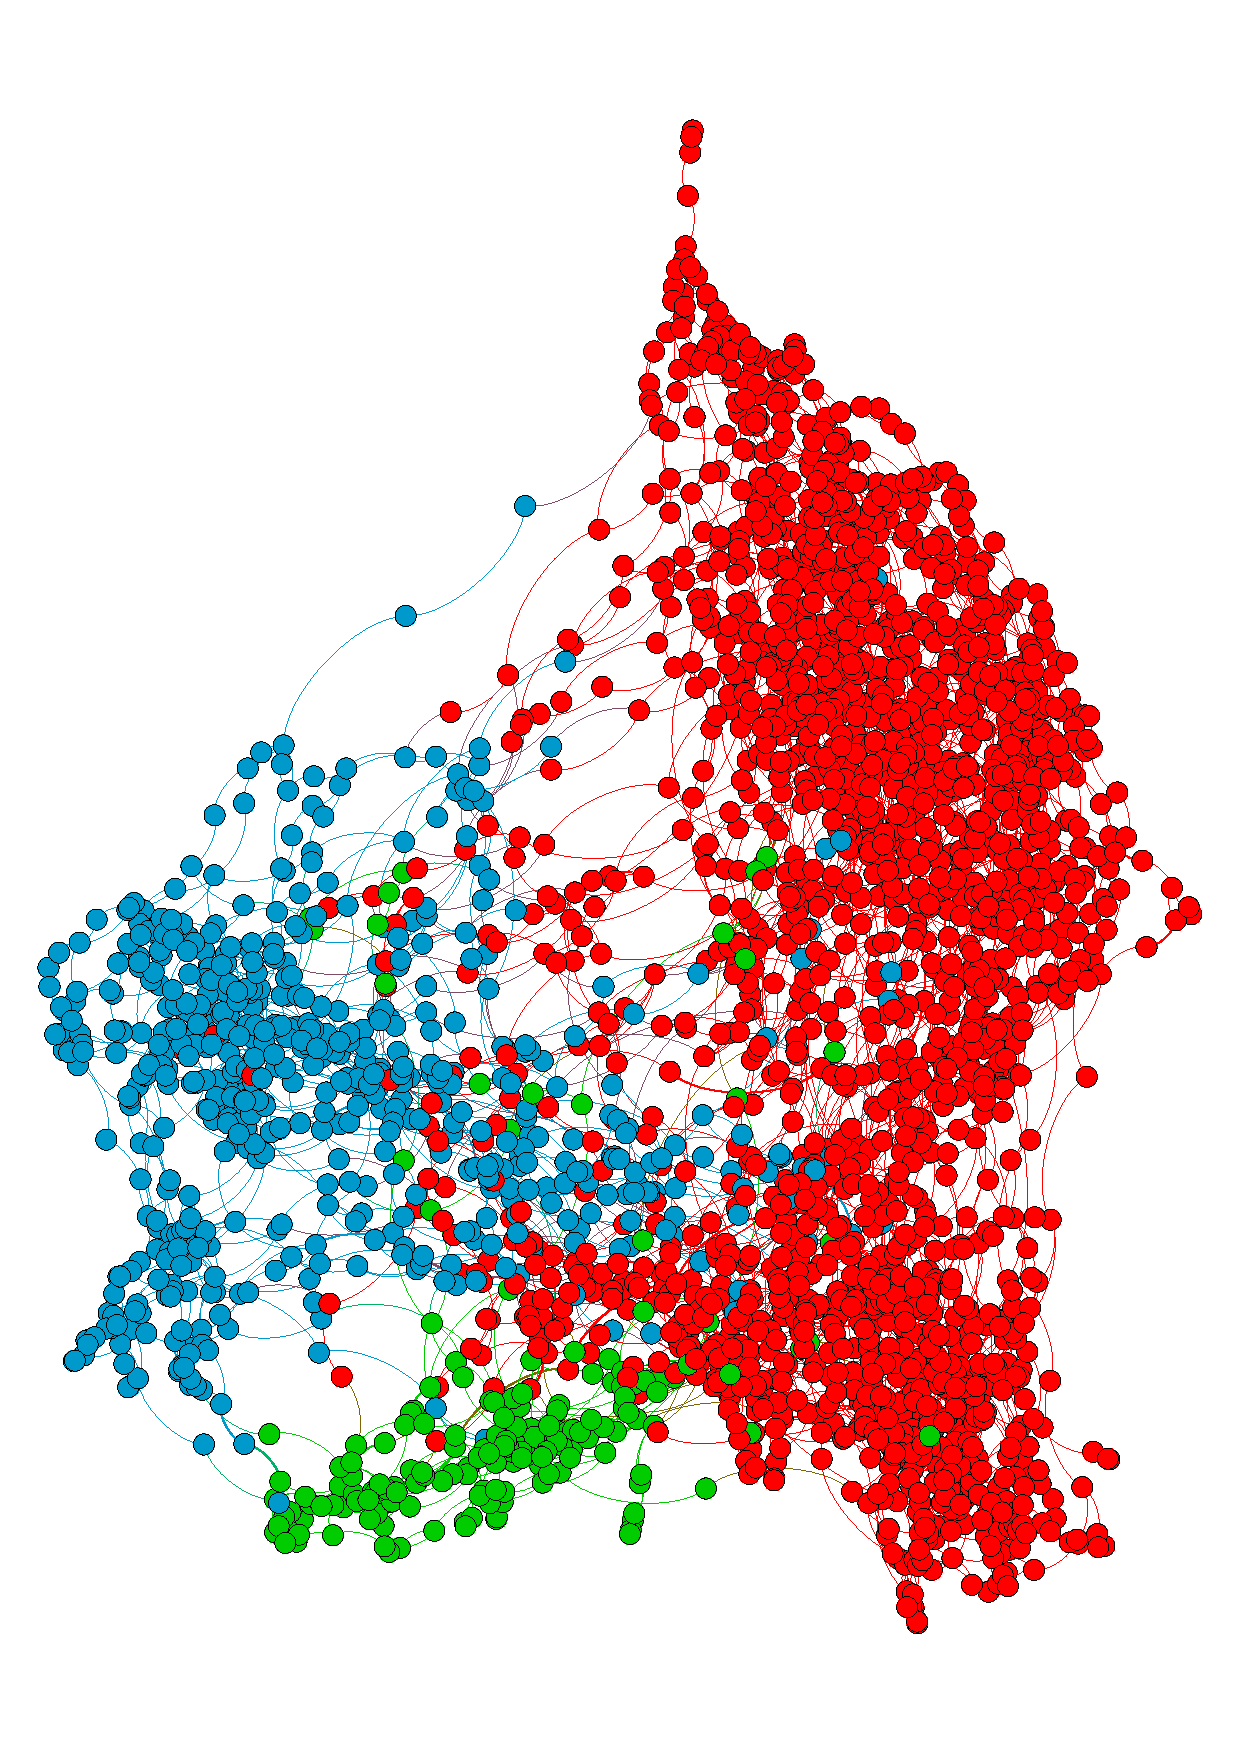
\includegraphics[width=1.7in]{Int2-3.pdf}
\label{fig:PictureInt2-3}
}\hspace{2em}
\subfigure[\textbf{kNN2 VAT k=2 NR.} Red nodes denotes C0, and Blue: C1.]
    {
        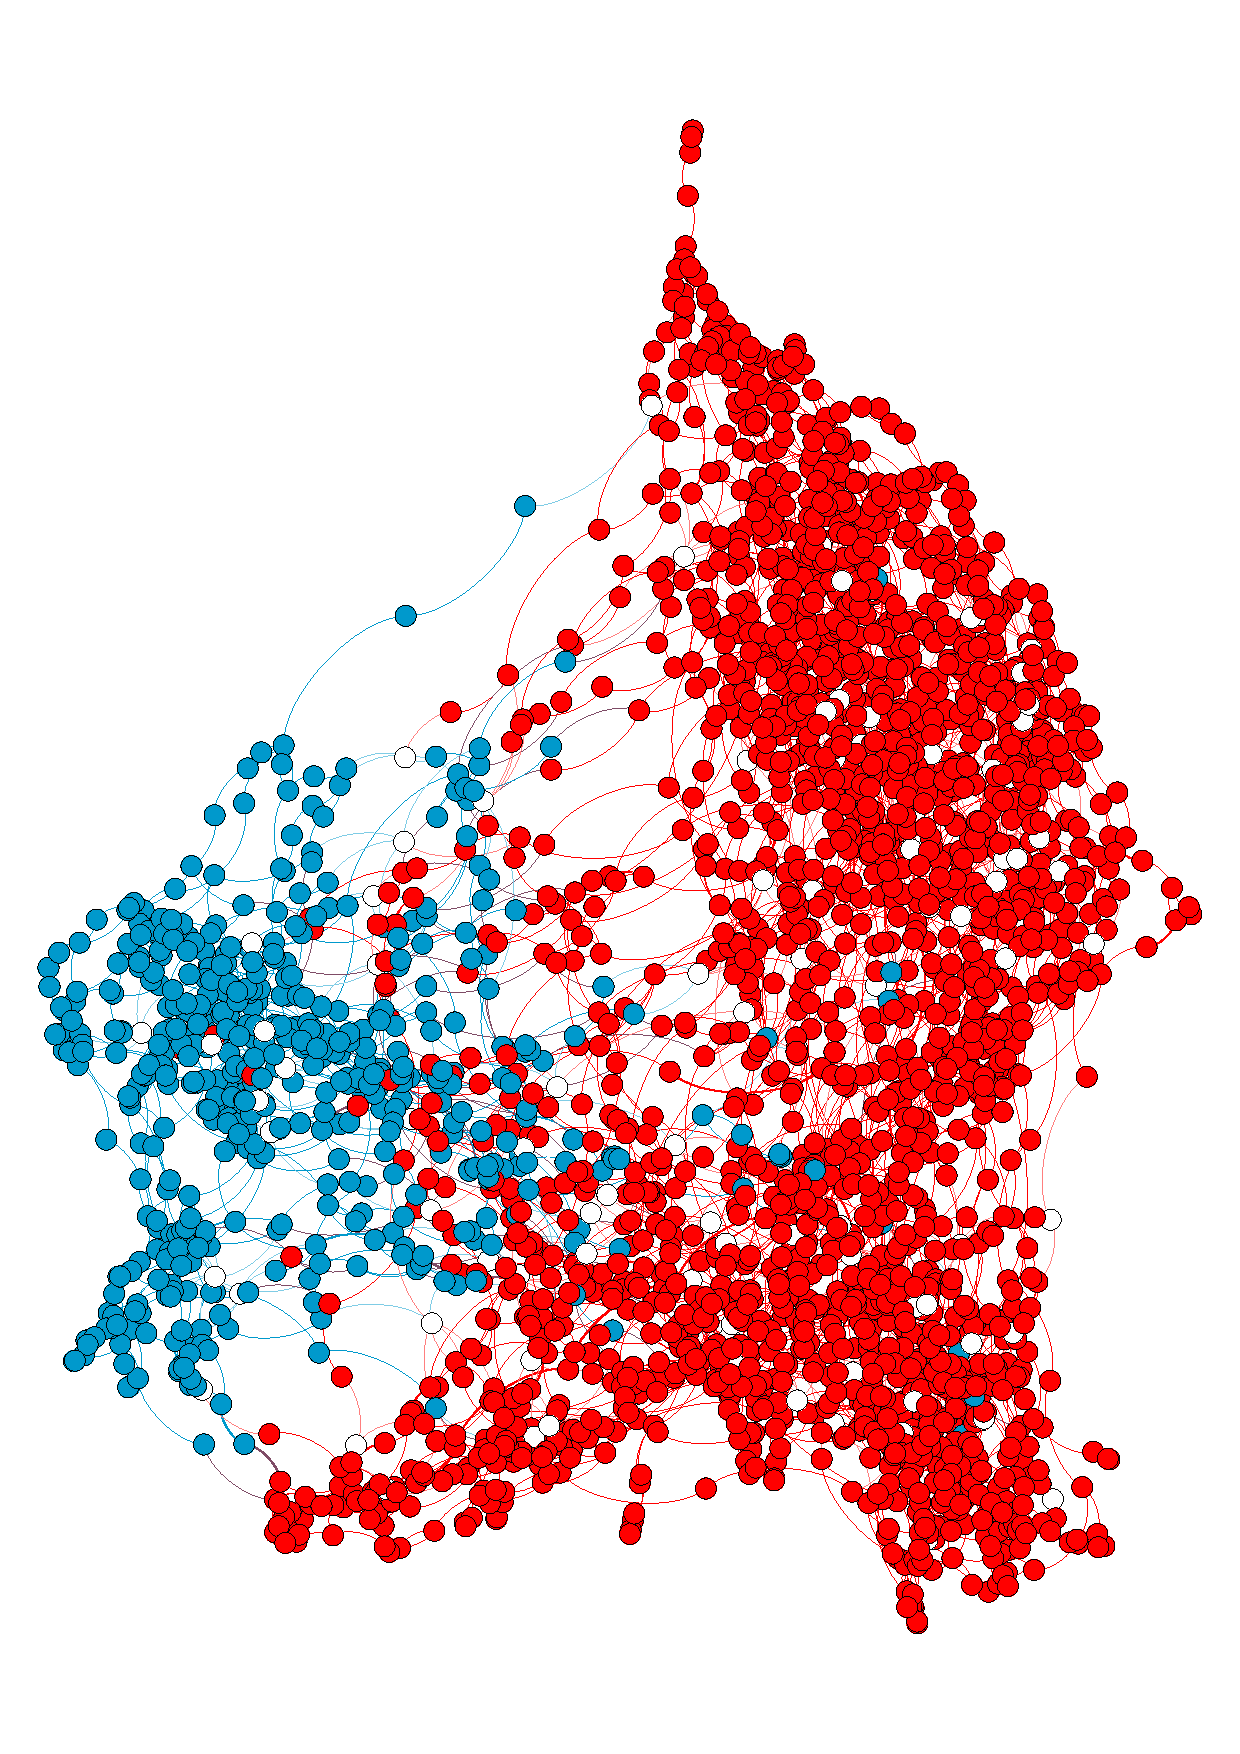
\includegraphics[width=1.8in]{VAT2-2NR.pdf}
        \label{fig:PictureVAT2-2NR}
    }\\
    \subfigure[\textbf{kNN2 VAT k=4.} Red nodes denotes C2, Blue: C3, Purple: C0, and Green: C1.]    
    {
        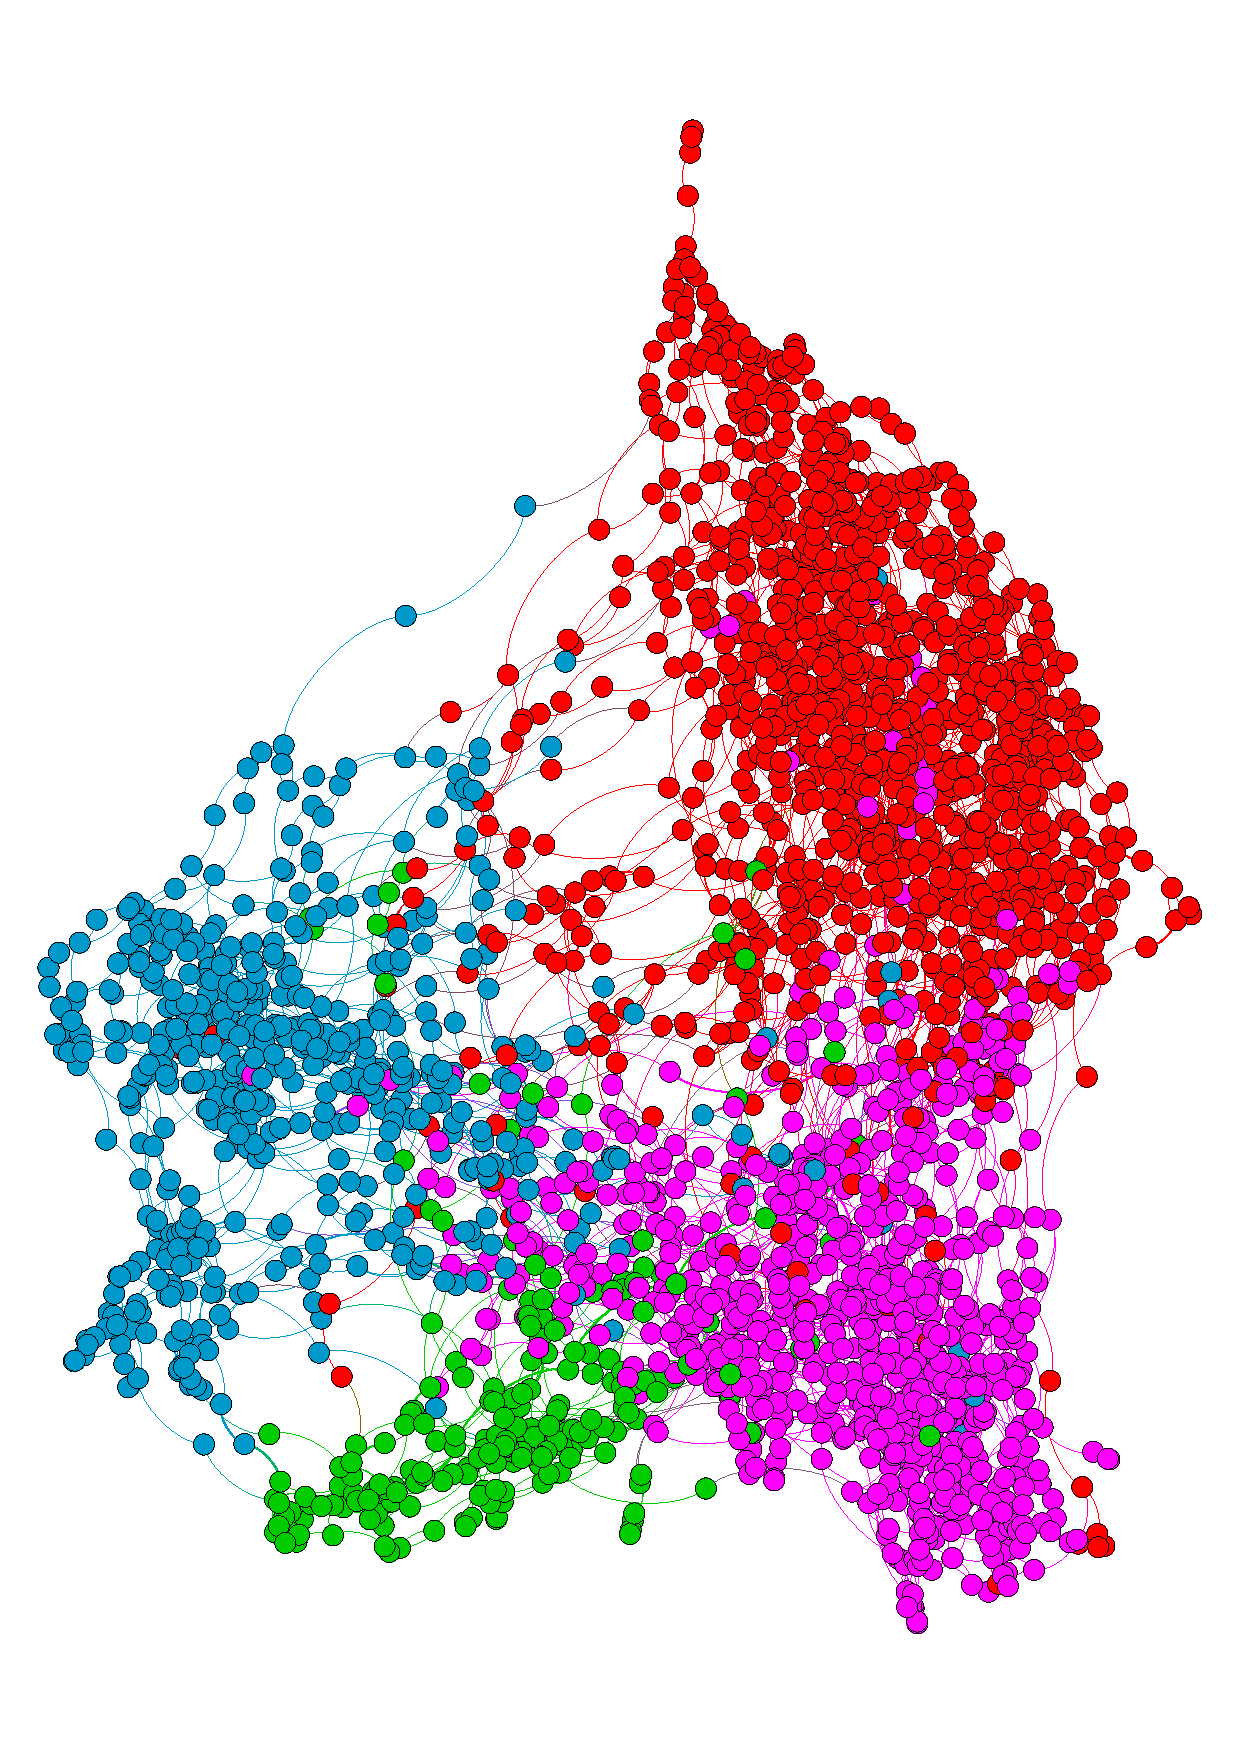
\includegraphics[width=1.8in]{VAT2-4.pdf}
        \label{fig:PictureVAT2-4}
    }\hspace{2em}
\subfigure[\textbf{kNN2 Integrity k=5 NR.} Red nodes denotes C0, Blue: C2, Gold: C1, Purple: C3, and Green: C4. ] 
    {
        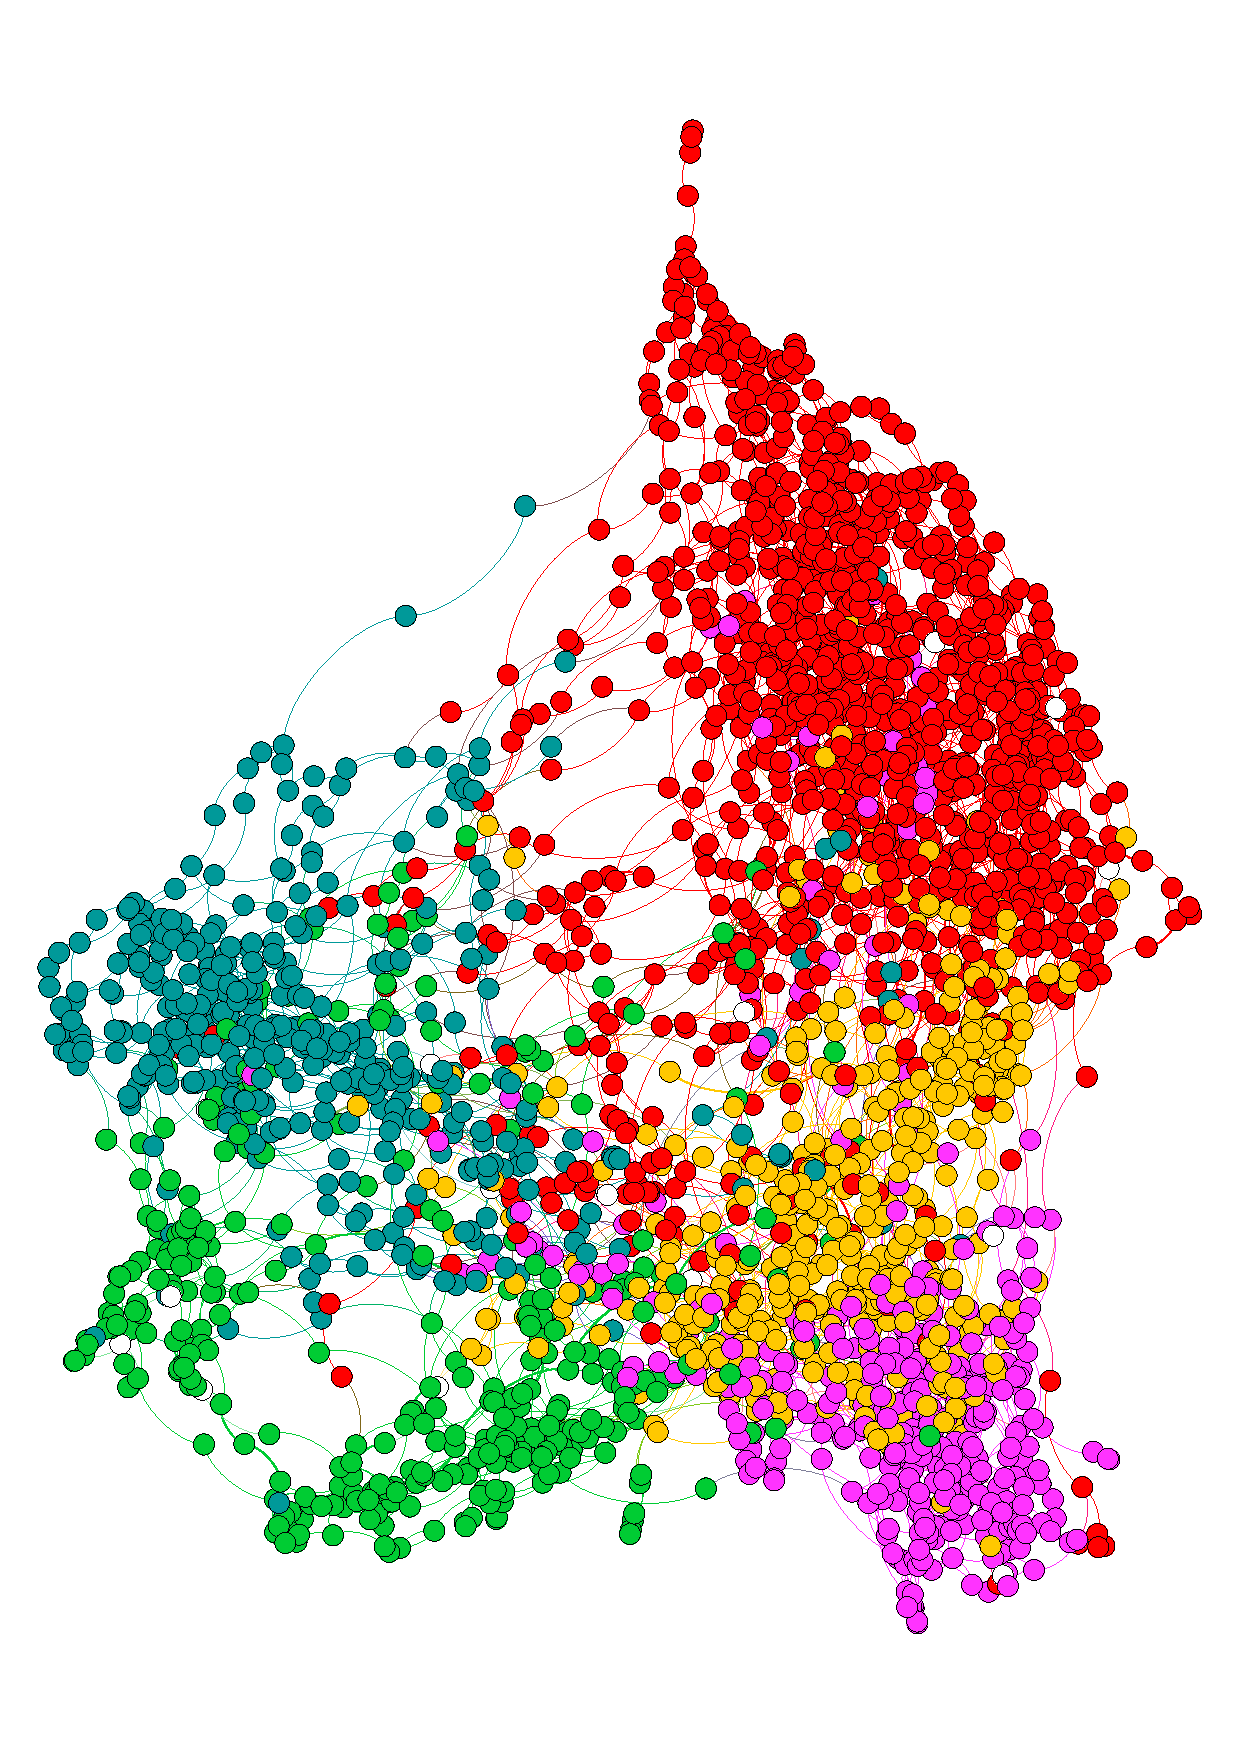
\includegraphics[width=1.7in]{Int2-5NR.pdf}
        \label{fig:PictureInt2-5}
    } 
\\
\subfigure[\textbf{kNN2 Tenacity k=5.} Red nodes denotes C2, Blue: C3, Gold: C0, Purple: C1, and Green: C4.]    
    {        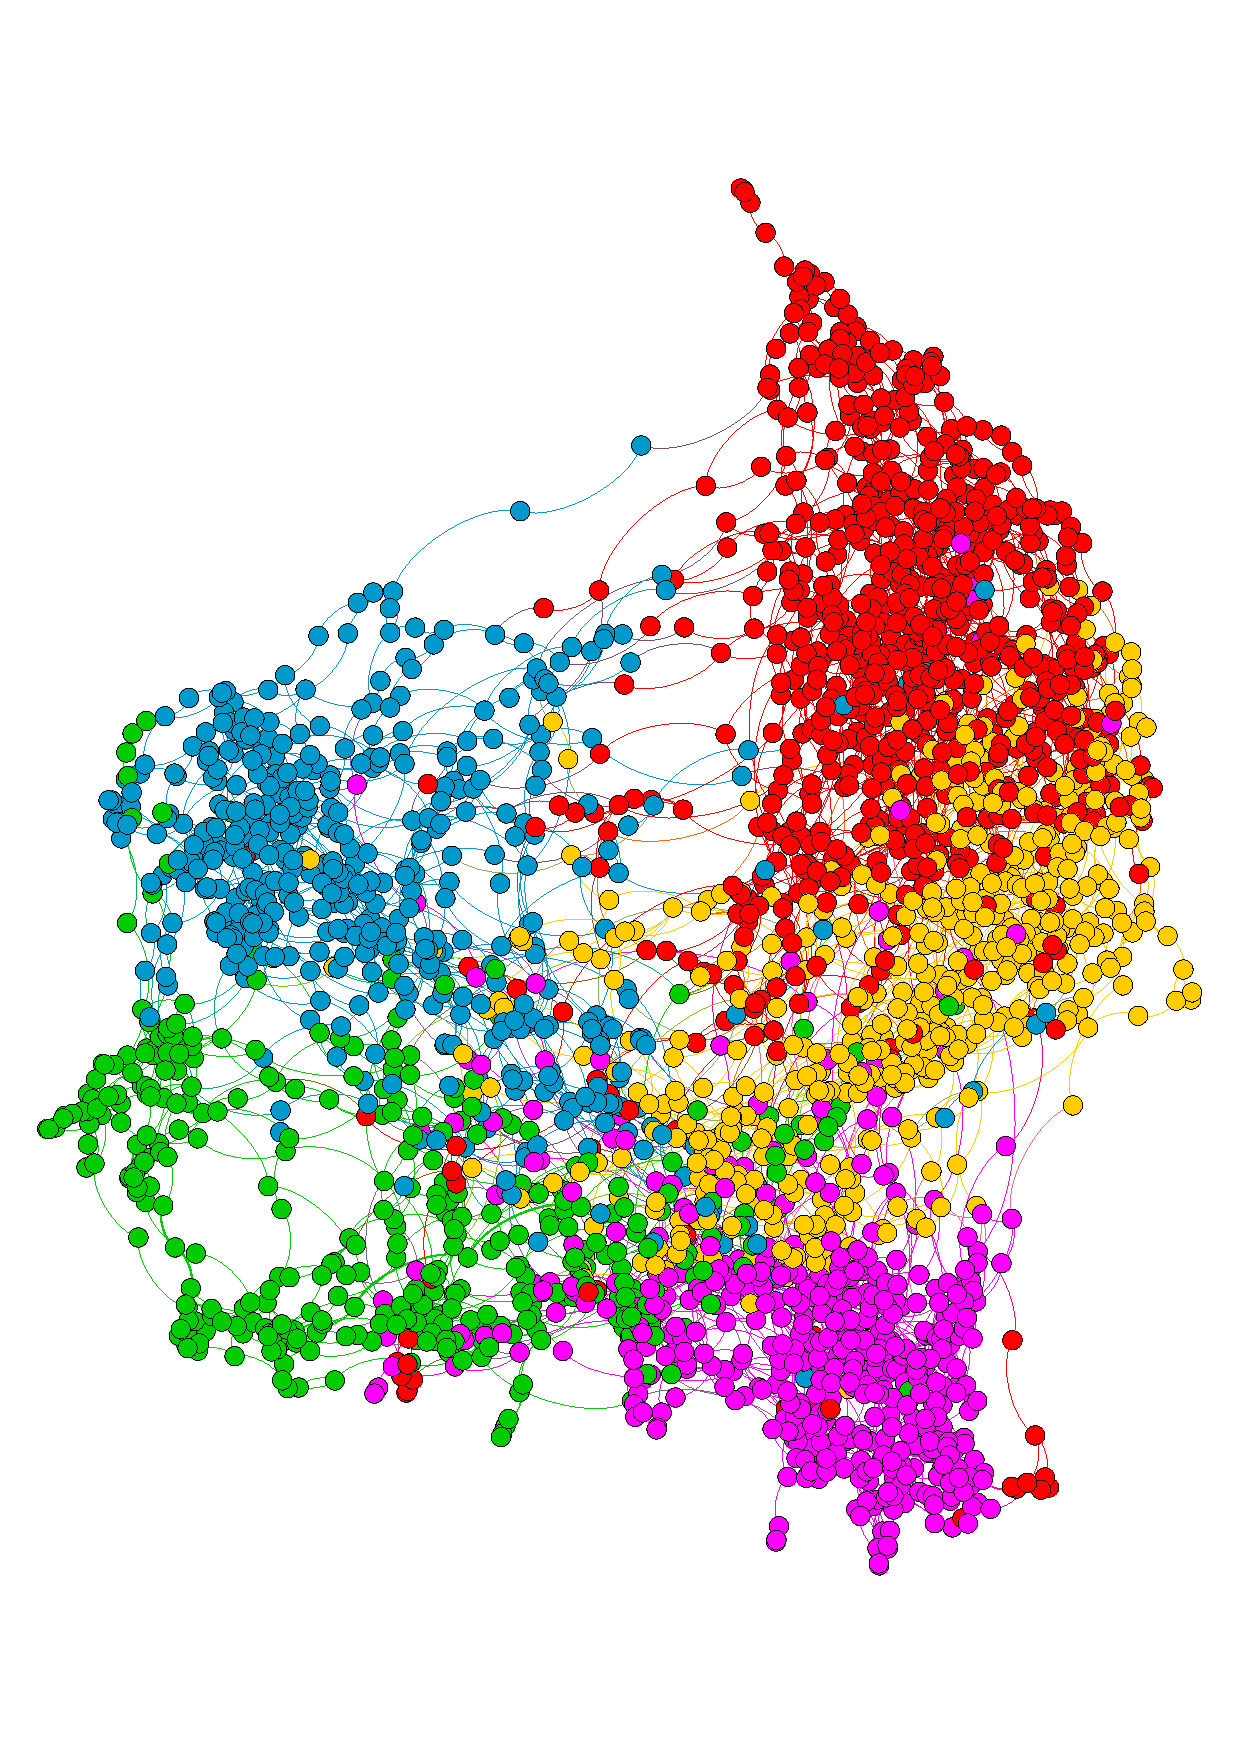
\includegraphics[width=1.7in]{TEN2-5.pdf}
        \label{fig:PictureTen2-5}
    }\hspace{2em}
\subfigure[\textbf{kNN2 Tenacity k=5 NR.} Red nodes denotes C1, Blue: C2, Gold: C3, Purple: C0, and Green: C4.]    
    {        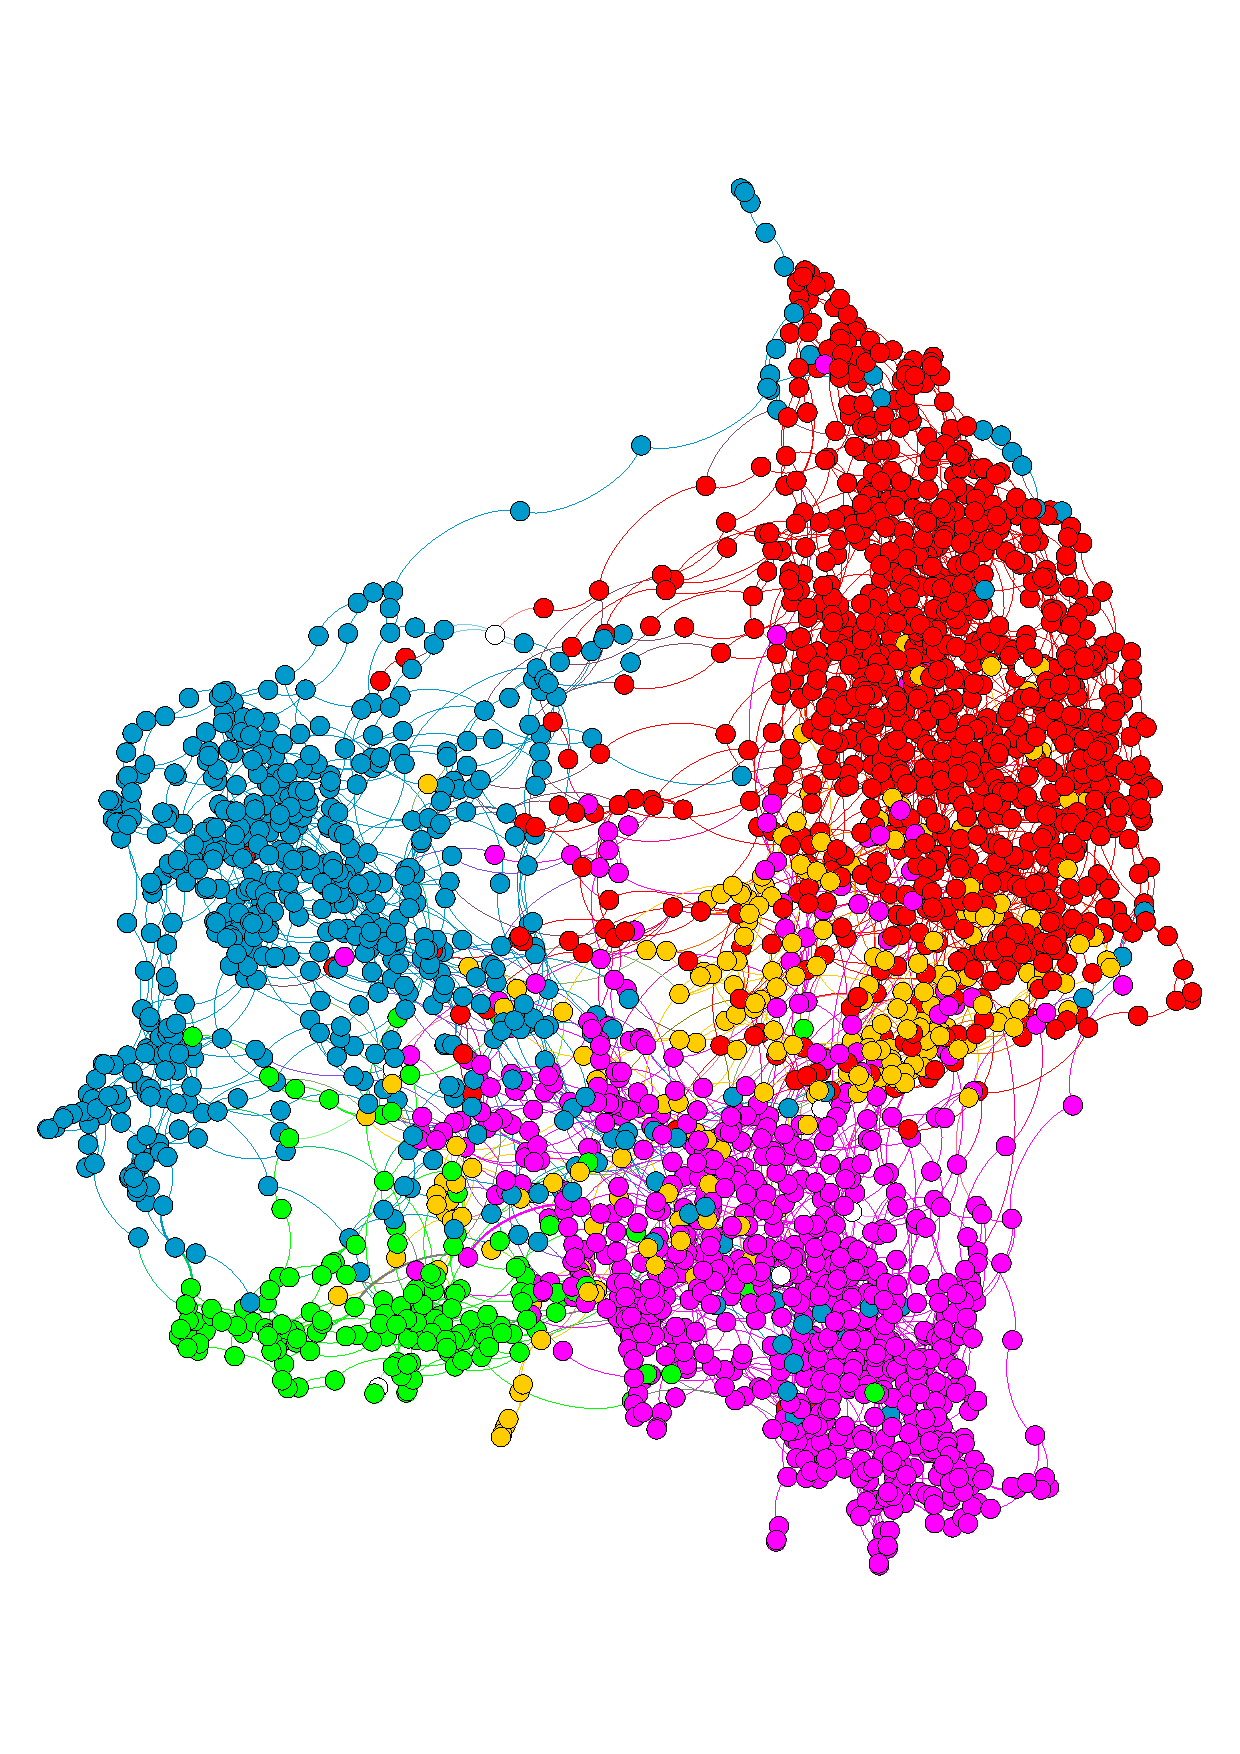
\includegraphics[width=1.7in]{TEN2-5NR.pdf}
        \label{fig:PictureTen2-5NR}
    }
\caption[]{Visualization of optimal clustering results by resilience measure. NR indicates no reassignment of attack set nodes.}
    \label{fig:NormalizationCharts}
\end{figure}


\begin{figure}
    \centering
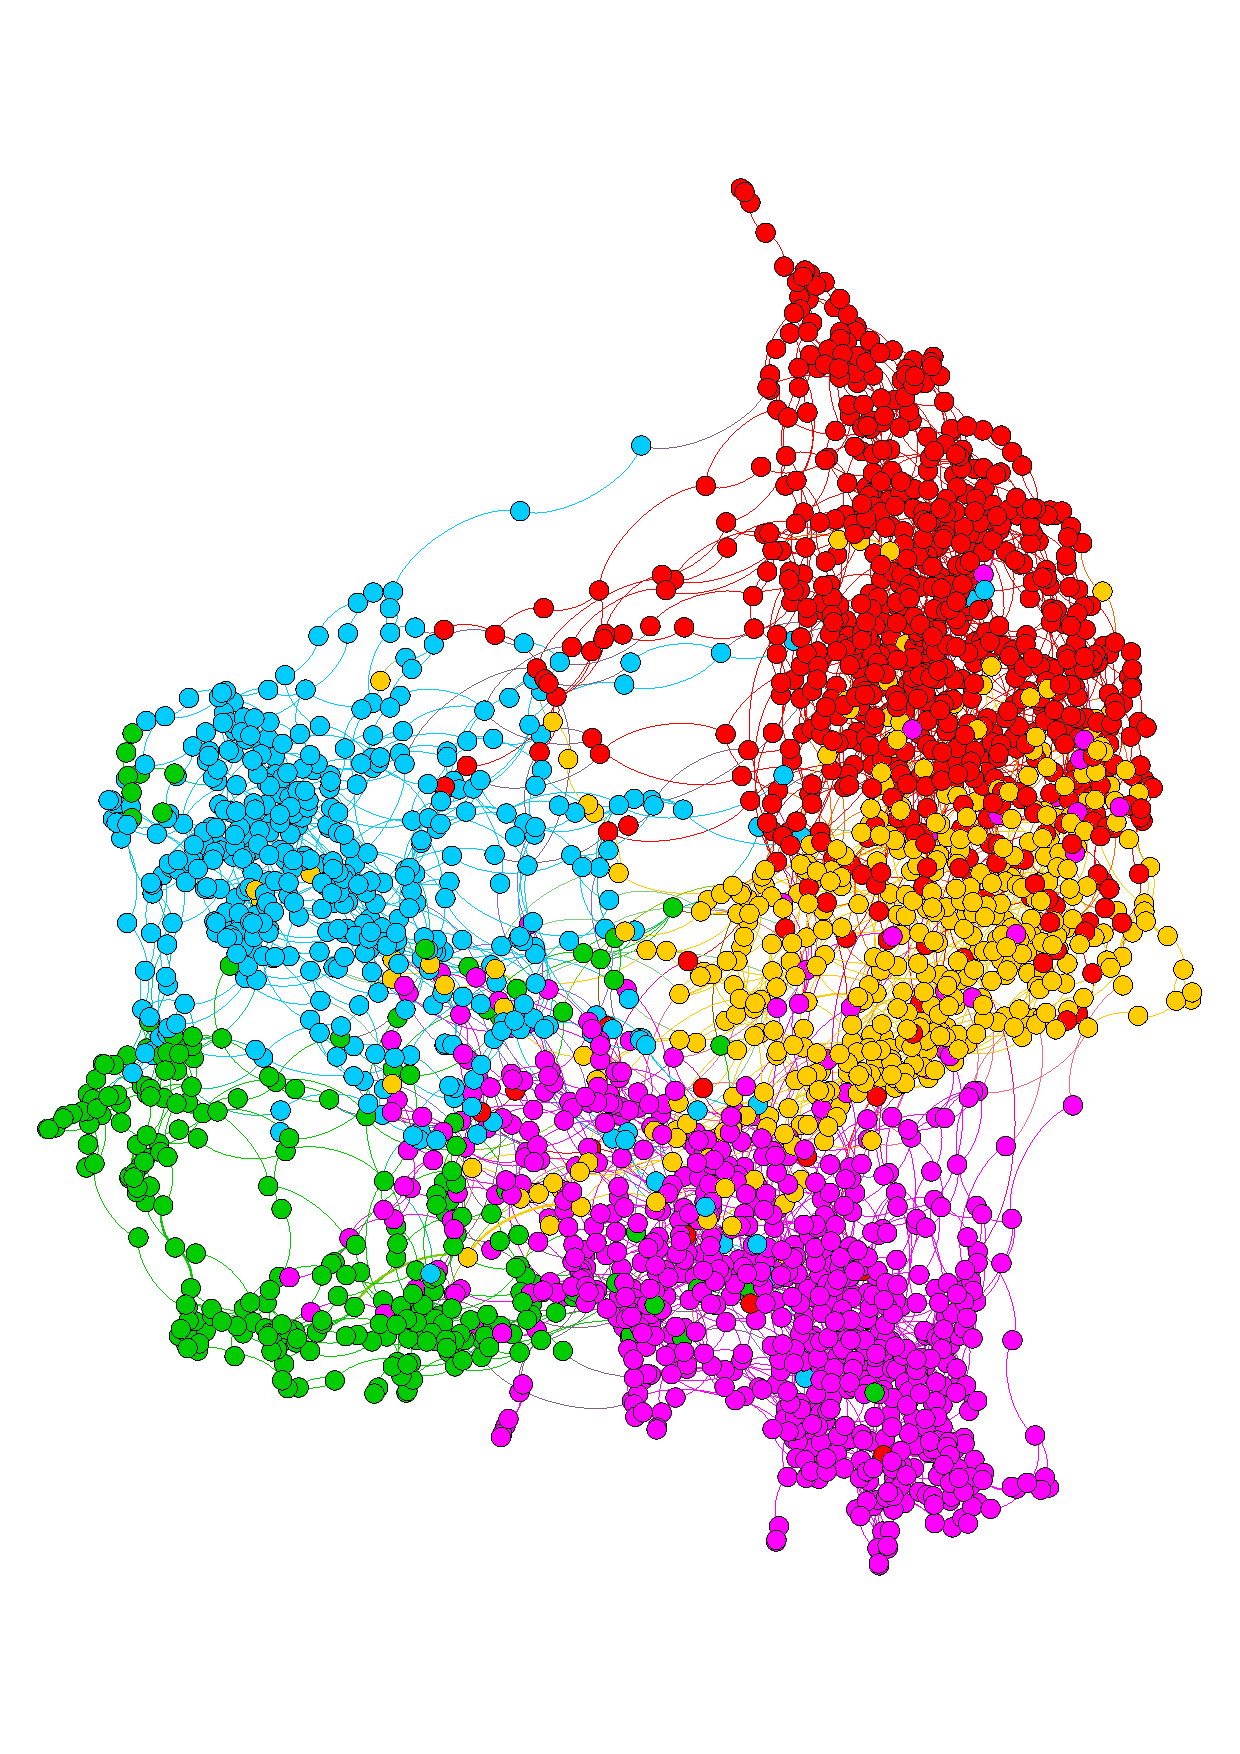
\includegraphics[width=2in]{Int3-5Cor8OrigForceAtlas.pdf}

\caption[]{Visualization of the graph of k=5 optimal clustering result for kNN3 with Integrity using the correlated filtered set. Red nodes denotes C2, Blue: C4, Gold: C0, Purple: C3, and Green: C1.}
\label{fig:Int35Cor8}
\end{figure}




The demographics (mean age at ADOS, ethnicity as quantified by percentage Caucasian, and gender) of each cluster of the optimal clustering configurations are shown in Tables \ref{tab:demoNodeReassignment} and \ref{tab:demoWithoutNodeReassignment}. We observe that there are no significant differences in the demographics across clusters for age and gender distribution. However, the distribution of percentage Caucasian varied across clusters.



\begin{table}[t]
  \caption{Demographics per cluster configuration with node reassignment}
  \label{tab:demoNodeReassignment}
  \centering
 % \noindent  %\adjustbox{max width=17cm}{%
 \resizebox{\textwidth}{!}{%
 \begin{tabular}{l|ccc|cccc|ccccc}
    \hline
    \multirow{2}{1cm}{ } &\multicolumn{3}{c|}{\rule{0pt}{3ex}Integrity k=3 } & \multicolumn{4}{c|}{VAT k=4}      &   \multicolumn{5}{c}{Tenacity k=5 } \\
   % {} &   {} &$N=70$ &  {}  &  {} & $N=69$ &  {}  &  {} & $N=71$ &  {}    \\
    {} &    C0     & C1		& 	C2	& 	C0     & C1		& 	C2	&C3 &	C0  & C1		& 	C2	&C3  & C4\\             
    \hline
\rule{0pt}{3ex}Mean Age&9.0	&8.4	&8.5		&8.9	&8.6	&8.9	&8.6		&9.0	&9.0	&8.9	&8.6	&8.6\\
\% Caucasian	&81.0	&64.5	&73.3		&78.3	&64.4	&83.9	&71.5		&82.6	&77.5	&83.7	&71.90	&69.3\\
 \% Male	&86.4	&84.1	&87.2		&87.2	&84.9	&85.8	&87.2		&85.4	&89.7	&86.6	&87.4	&82.0\\

    \hline
  \end{tabular}
  }%end resizebox
\end{table} 

\begin{table}[t]
  \caption{Demographics per cluster configuration without node reassignment. }
  \label{tab:demoWithoutNodeReassignment}
  \centering
 % \noindent  %\adjustbox{max width=17cm}{%
 \resizebox{\textwidth}{!}{%
 \begin{tabular}{l|cccccc|cccccc|ccc}
    \hline
    \multirow{2}{1cm}{ } &\multicolumn{6}{c|}{\rule{0pt}{3ex}kNN2 Tenacity k=5  } & \multicolumn{6}{c|}{kNN2 Integrity k=5}      &   \multicolumn{3}{c}{kNN2 VAT k=2 } \\
   % {} &   {} &$N=70$ &  {}  &  {} & $N=69$ &  {}  &  {} & $N=71$ &  {}    \\
    {} &    C0     & C1		& 	C2	& 	C3     & C4	 & S	& 	C0	&C1 &	C2  & C3		& 	C4	&S  &C0  & C1 &S\\             
    \hline
\rule{0pt}{3ex}Mean Age 	&	8.8	&	9.0	&	8.7	&	8.9	&	8.6	&	9.32& 8.9	&	8.8	&	8.7	&	9.3	&	8.4	& 9.6&	8.9	&	8.6 & 8.6 \\
\% Caucasian	&	78.7&	85.3	&	71.1	&	74.5	&	64.5 &77.8	&	83.8	&	77.4	&	71.6	&	79.3	&	67.2	&83.3 &	79.9	&	71.7 & 74.5\\
 \% Male	&	88.3&	85.3&	86.3	&	86.1	&	84.9	& 100.0&	86.0&	85.1	&	87.3&	88.5	&	85.4	&94.4 &	86.1	&	87.2 & 90.2
\\
    \hline
  \end{tabular}
  }%end resizebox
\end{table} 



Statistical analyses of the optimal clustering configurations for each ASD outcome measures are presented in Tables~\ref{tab:autismTableWithNR} and~\ref{tab:autismTableWithoutNR}. Note that for the no node reassignment results (Table~\ref{tab:autismTableWithoutNR}), though the mean and standard deviation values for $S$ is reported for each outcome measure, it is excluded from the Anova, Tukey and Eta-squared analysis. Higher values of ADOS CSS, RBS, ABC and SRS scores implies greater ASD severity levels while higher values of full scale IQ, Vineland composite, and PPVT 4A scores implies lesser ASD severity levels. (The cohen effect size pairwise comparison results are included as a supplementary file.)
We can observe that the overall effect sizes, as quantified by the $\eta^2$ value is consistently high for  kNN2 Tenacity 5-Cluster result in Table \ref{tab:autismTableWithNR}. Cluster C4 appears to be the most severe ASD subgrouping in terms of low overall IQ, relatively high occurrence epilepsy (non-febrile seizures), low functioning skills (as quantified by the Vineland composite scores), and high ADOS CSS scores. However, their ABC and RBS-R scores are not the most severe scores, and are slightly better compared to cluster C0. Cluster C0 has very high mean IQ scores (not the highest - C2), but the ABC and RBS-R scores for that subgroup are the lowest. %This provides further evidence that there is an ASD subgroup with relatively IQ scores but very severe behavioral problems \cite{obafemi2015sorting}. 
For the no node reassignment analysis (Table~\ref{tab:autismTableWithoutNR}), the 2-cluster VAT-clust result does not seem to convey much practical significance based on the relatively low $\eta^2$ values across all ASD outcome measures evaluated.

Figure~\ref{fig:knn2Ten5IQresult} illustrates the visualization of the graph of the optimal clustering result for kNN2 Tenacity 5-Cluster results in terms of distribution of high overall IQ ($\geq 70$) vs. lower IQ ($<70$). Large circles denote high IQ while small circles denote low IQ. Only the green cluster (C4) shows a high concentration of low IQ nodes (small circles).  We can observe the complexity of the variation in the 5-cluster result given by Tenacity kNN2 with node reassignment. This demonstrates that the resulting clustering obtained is a combination of various factors, not just IQ scores. 


%We also observe that the Integrity 5-cluster result is similar to the kNN2 Tenacity 5-Cluster node reassignment result (Table~\ref{tab:autismTableWithNR}).} 

%The clinical evaluation appears meaningful as in every case one cluster has a lower mean Overall IQ, lower Vineland composite Score (which signifies adaptive functioning), and lower Learning Vocabulary Score (PPVTA), as well as a higher incidence of epilepsy.  
%This clustering is atypical, as its least-affected cluster has 743 nodes and is not largest. A second cluster of 462 nodes also has high Overall IQ, Vineland Composite Score, Learning Vocabulary Score (PPVTA), and the lowest incidence of epilepsy. The largest cluster C3 at 744 nodes ranks third, although the measures for C3 and C4 are very similar.  In fact, clusters C3 and C4 are identified by Tukey HSD as similar for 5 of 7 measures. 

\begin{table}[tbp]
\centering
\caption{Statistical analysis of optimal clustering configurations (complete clustering) by graph type and node resilience measure using selected ASD outcome measures. The mean and standard deviation values are presented for each measure.}
\label{tab:autismTableWithNR}
\resizebox{\textwidth}{!}{%
\begin{tabular}{l|ccccccc}

Cluster (\textbf{size})   & \makecell{ABC\\Overall} & \makecell{RBS R\\Overall}  & \makecell{ADOS \\CSS}    & \makecell{Vineland \\Composite \\Score} & Overall IQ & PPVTA 4A& \makecell{Epilepsy }   \\ \hline
                                                                      
\multicolumn{7}{c}{\rule{0pt}{3ex}kNN 2 Integrity k=3 }  \\                                                                              C0 (1903)	&45.73(25.8)	&27.31(18.1)	&7.37(1.7)	&75.72(10.9)	&88.19(23.5)	&91.51(24.7)	&	1.74\%\\
C1 (189)	&54.08(24.6)	&29.01(13.8)	&7.58(1.5)	&57.57(9.6)	&38.91(18.7)	&41.75(22.3)	&	6.91\%\\
C2 (588)	&47.55(25.9)	&26.26(16.3)	&7.63(1.6)	&70.58(12.3)	&69.99(27.6)	&72.41(28.8)	&	2.73\%\\
ANOVA p-value & $<0.001$ & $ 0.15$ & $ 0.003$ & $<0.001$ & $<0.001$ & $<0.001$\\				
Tukey HSD (NS$\dagger$) &C0:C2& all pairs & C1:C0,C2 & none & none & none\\				
Eta-squared ($\eta^2$) & 0.007 & 0.001 & 0.004& 0.157 & 0.244 & 0.209  & \\				
\hline

\multicolumn{7}{c}{\rule{0pt}{3ex}kNN 2 VAT k=4 }     \\  
C0 (811)	& 50.86 (28.0)	& 31.76 (19.6)	& 7.48 (1.7)	& 72.69 (10.3)	& 80.06 (22.8)	& 82.98 (24.1)	&	2.47\%\\
C1 (219)	& 60.02 (28.5)	& 32.33 (17.4)	& 7.68 (1.5)	& 57.74 (9.4)	& 39.55 (18.7)	& 41.93 (21.3)	&	5.99\%\\
C2 (1117)	& 41.55 (22.2)	& 23.89 (15.4)	& 7.24 (1.7)	& 78.16 (10.4)	& 94.77 (20.8)	& 98.34 (22.1)	&	1.25\%\\
C3 (535)	& 45.73 (25.2)	& 25.08 (16.0)	& 7.70 (1.6)	& 70.50 (12.8)	& 69.12 (28.2)	& 71.39 (29.1)	&	2.82\%\\
ANOVA p-value & $<0.001$ & $<0.001$ & $<0.001$ & $<0.001$ & $<0.001$ & $<0.001$\\			
Tukey HSD (NS$\dagger$) &none&C0:C1;C2:C3&\makecell{C0:C1,C3\\C1:C3}&none& none&none\\			
Eta-squared ($\eta^2$) & 0.047 & 0.046 & 0.013& 0.212& 0.322 & 0.288  & \\			

\hline

\multicolumn{7}{c}{\rule{0pt}{3ex}kNN 2 Tenacity k=5}  \\                                                                                  C0 (535)  &67.12(21.5)    &41.78(18.2)   &7.30(1.7)  &73.71(9.7)	  &91.46(21.6)	  &96.46 (23.8)	  &1.31 \%\\
C1 (497)	&36.57(19.6)	&22.10(12.6)	&7.40(1.6)	&74.56(10.2)	&80.65(22.5)	&82.57 (23.4)	&2.42\%\\
C2 (781)	&33.78(19.3)	&18.34(11.4)	&7.22(1.7)	&78.85(11.0)	&92.99(22.8)	&96.59(22.9)	&1.41\%\\
C3 (484)	&44.05(23.9)	&25.35(15.5)	&7.58(1.7)	&74.29(11.0)	&79.31(23.7)	&81.04(24.4)	&2.07\%\\
C4 (383)	&61.19(27.5)	&33.83(18.9)	&7.97(1.5)	&58.62(9.5) 	&42.20(19.4)	&44.86(22.8)	&5.76\%\\
ANOVA p-value & $<0.001$ & $<0.001$ & $<0.001$ & $<0.001$ & $<0.001$ & $<0.001$\\
Tukey HSD (NS$\dagger$) &C1:C2 & none &\makecell{C0:C1,C2,C3\\C1:C2,C3}
&\makecell{C0:C1,C3\\C1:C3}&C0:C2;C1:C3&C0:C2;C1:C3\\
Eta-squared ($\eta^2$) & 0.274	&0.253	&0.022 &	0.272&	0.361 &0.333
\\
\hline
\multicolumn{7}{c}{\rule{0pt}{3ex}kNN 3 Integrity k=5 corr}                         \\                                                   
C0 (462)	&66.56(24.0)	&41.65(18.3)	&7.54(1.7)	&73.26(9.6)	&87.95(22.9)	&92.57(24.5)		&0.87\%\\
C1 (276)	&57.20(27.4)	&29.89(15.5)	&7.39(1.4)	&57.38(8.9)	&37.27(17.8)	&39.84(21.8)		&5.82\%\\
C2 (743)	&33.48(18.7)	&17.39(10.6)	&7.18(1.7)	&79.86(10.6)	&96.22(20.6)	&99.49(21.6)		&1.62\%\\
C3 (744)	&46.25(24.8)	&28.80(17.8)	&7.53(1.6)	&72.53(10.4)	&78.72(23.3)	&80.97(24.9)		&3.10\%\\
C4 (455)	&42.58(23.2)	&24.26(14.9)	&7.66(1.8)	&73.63(12.0)	&77.54(25.2)	&79.01(26.2)		&1.54\%\\ 
ANOVA p-value & $<0.001$ & $<0.001$ & $<0.001$ & $<0.001$ & $<0.001$ & $<0.001$\\				
Tukey HSD (NS$\dagger$) &C3:C4&C1:C3& \makecell{ C0:C1,C3,C4\\C1:C2,C3,C4\\C3:C4}& \makecell{C0:C3,C4\\C3:C4}&C3:C4&C3:C4\\				
Eta-squared ($\eta^2$) & 0.197& 0.215 & 0.011& 0.258 & 0.354 & 0.306  & \\				
\hline

\end{tabular}
}%end resizebox
\begin{tablenotes}\footnotesize
\item $\dagger$NS: implies pairs for which Tukey HSD test was not significant.

\end{tablenotes}
\end{table}

\begin{table}[tbp]
\centering
\caption{Statistical analysis of optimal clustering configurations using selected ASD outcome measures: for kNN2 graphs without node reassignment. The mean and standard deviation values are presented for each measure.)}
\label{tab:autismTableWithoutNR}
\renewcommand{\arraystretch}{1}
\resizebox{\textwidth}{!}{%
\begin{tabular}{l|lllllll}
Cluster (\textbf{size})   & \makecell{ABC\\Overall} & \makecell{RBS R\\Overall}  & \makecell{ADOS \\CSS}    & \makecell{Vineland \\Composite \\Score} & Overall IQ & PPVTA 4A& \makecell{Epilepsy } \\ \hline
                                                                      
\multicolumn{7}{c}{\rule{0pt}{3ex}kNN 2 VAT k=2 }    \\                                                                             
C0 (2072)	&47.01(26.1)	&27.74(17.9)	&7.38(1.7)	&73.99(12.0)	&83.50(27.1)	&87.51(27.9)	&	2.27\%\\
C1 (506)   &45.66(25.3)	  &25.01(16.1)	&7.69(1.6)	&70.47(12.9)	&69.09(28.5)	&71.46(29.3)	&	2.77\%\\
S (102) &46.03(21.6)&26.89(15.1)&7.52(1.5)&73.71(9.6)&81.75(23.2)&77.94(35.1)&0.98\%\\
ANOVA p-value & $0.295$ & $0.002$ & $<0.001$ & $<0.001$ & $<0.001$ & $<0.001$\\							
Eta-squared ($\eta^2$)&	0	&0.004	&0.005	&0.013	&0.042	& 0.049												
\\ \hline                           
\multicolumn{7}{c}{\rule{0pt}{3ex}kNN 2 Integrity k=5 }     \\                                                                             
C0 (1096)	&41.02(22.0)	&23.30(14.8)	&7.19(1.7)	&78.36(10.3)	&94.63(20.6)	&97.91(22.2)	&	1.37\%\\
C1 (430)	&67.76(24.6)	&43.94(19.2)	&7.61(1.7)	&70.22(9.7)	&78.58(23.8)	&83.02(25.0)	&	1.86\%\\
C2 (402)	&41.49(23.8)	&24.42(15.8)	&7.57(1.7)	&73.88(11.3)	&78.34(24.3)	&79.36(25.4)	&	2.00\%\\
C3 (384)	&32.54(18.1)	&18.99(10.5)	&7.47(1.6)	&75.41(10.6)	&82.90(21.9)	&84.73(23.3)	&	2.09\%\\
C4 (350)	&59.67(27.2)	&30.74(17.2)	&7.83(1.5)	&58.58(9.9)	  &40.55(19.3)	&43.70(22.9)	&	6.03\%\\ 
\textbf{S (18) }     &56.33(22.6)    &32.50(15.0)    &7.72(1.9)  &69.33(14.2)  &68.78(36.4)  &65.56(46.7)    &  11.1\%\\

ANOVA p-value & $<0.001$ & $<0.001$ & $<0.001$ & $<0.001$ & $<0.001$ & $<0.001$\\								
Tukey HSD (NS$\dagger$) &C0:C2  & C0:C2 & \makecell[l]{C1:C2,C3,C4;\\C2:C3,C4} & C2:C3 &C1:C2 & C1:C2,C3\\								
Eta-squared ($\eta^2$) &0.211	&0.210	&0.019	&0.279	&\textbf{0.383}	&0.329	\\		
\hline
\multicolumn{7}{c}{\rule{0pt}{3ex}kNN 2 Tenacity k=5}       \\                                                                             
C0 (741)	&47.01(26.1)	&29.38(18.8)	&7.46(1.6)	&73.25(9.9)	&81.26(22.4)	&83.63(23.3)	&	2.30\%\\
C1 (951)	&41.23(22.4)	&22.84(14.8)	&7.08(1.7)	&78.68(10.5)	&95.58(20.3)	&99.41(21.6)	&	1.26\%\\
C2 (591)	&45.06(26.3)	&25.66(17.3)	&7.61(1.7)	&71.44(13.3)	&70.86(28.5)	&72.95(29.9)	&	2.54\%\\
C3 (216)	&68.07(25.8)	&41.92(17.0)	&8.56(1.5)	&68.76(8.9)	&75.79(27.1)	&80.39(28.1)	&	2.33\%\\
C4 (172)	&54.72(25.2)	&28.90(14.0)	&7.35(1.4)	&56.13(8.9)	&36.17(16.6)	&37.64(18.6)	&	7.60\%\\
\textbf{S (9)}      &46.22(19.4)    &23.56(15.7)    &7.78(1.0)  &72.67(11.8) &79.00(23.5)   &81.88(34.3)   &   0\%\\
ANOVA p-value & $<0.001$ & $<0.001$ & $<0.001$ & $<0.001$ & $<0.001$ & $<0.001$\\					
Tukey HSD (NS$\dagger$)& C0:C2 & C4:C0,C2 & \makecell{C0:C2,C4\\ C4:C1,C2}& none& C2:C3 &C0:C3
\\					
Eta-squared ($\eta^2$) &0.078	&0.086	&0.054	&0.214	&\textbf{0.298}	&0.270\\
\hline 
\end{tabular}
} %end reesizebox
\begin{tablenotes}\footnotesize
\item $\dagger$NS: implies pairs for which Tukey HSD test was not significant. S is not included in the ANOVA, Tukey, and Eta-squared analyses.

\end{tablenotes}
\end{table}

\begin{figure}
    \centering
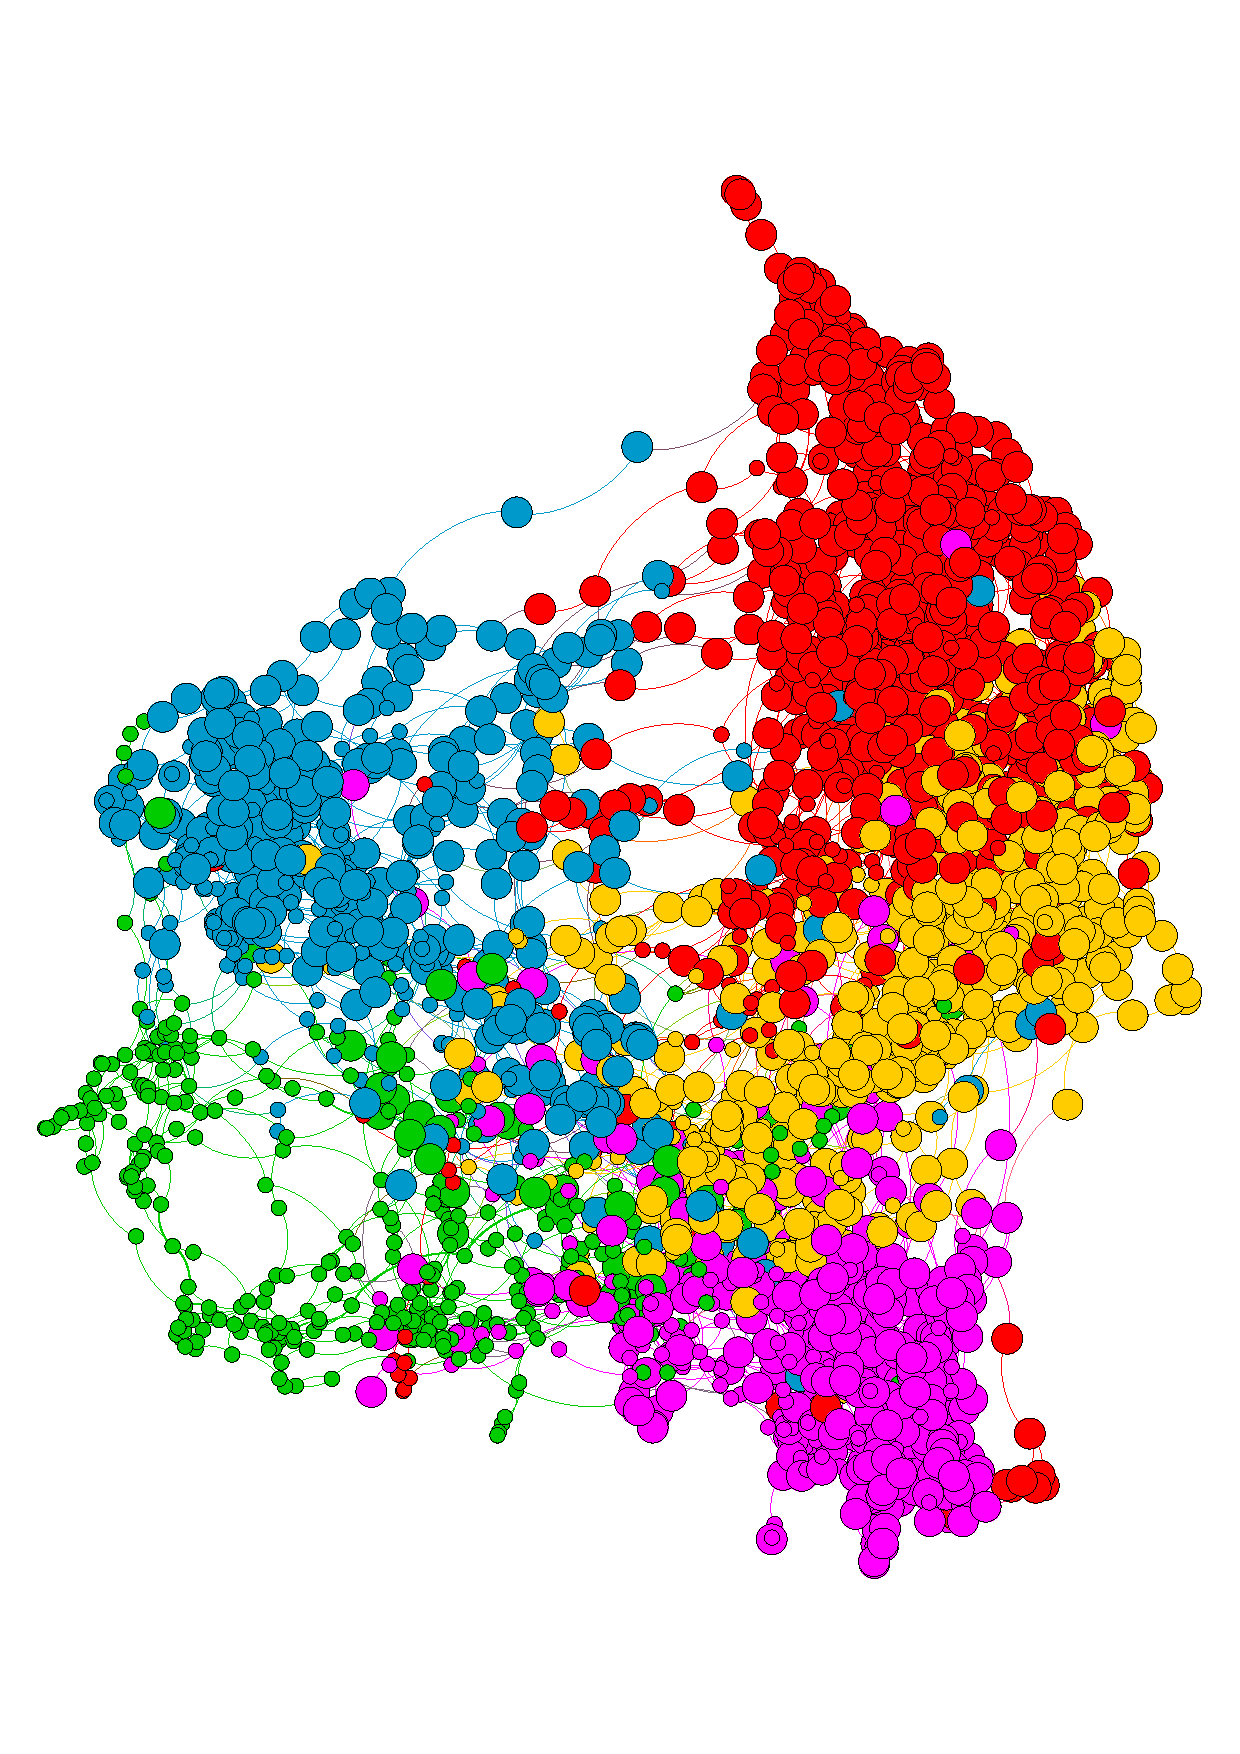
\includegraphics[width=3in]{IQUnder70Small.pdf}

\caption[]{Visualization of optimal clustering result for kNN2 Tenacity 5-cluster graph in terms of distribution of high overall IQ ($\geq 70$) vs. lower IQ ($<70$). Large circles denote high IQ while small circles denote low IQ. Only green cluster shows a high concentration of low IQ nodes. This demonstrates that the clustering obtained is a combination of various factors, not just IQ scores.}
\label{fig:knn2Ten5IQresult}
\end{figure}


The outcome of the feature extraction phase is summarized in Tables \ref{tab:featext} and \ref{tab:featextNR} for each of the seven clustering configurations.  Overall, 20 different features were uncovered as discriminant for at least one of the 7 optimal clusterings.  The regression feature was consistently selected for all seven results.  Overall level of language (ADI-R Q30) was selected six times while both BAPQ Mother overall average score and word delay were selected five times. 

\begin{table}[t]
  \caption{Set of discriminant features by clustering result for Complete Clustering Configuration}
  \label{tab:featext}
  \centering
 % \noindent  %\adjustbox{max width=17cm}{%
 \resizebox{\textwidth}{!}{%
\begin{tabular}{llll}
  \hline
    \makecell{Integrity\\k=3} & \makecell{Tenacity (corr)\\k=5}   & \makecell{VAT\\k=4} & \makecell{\rule{0pt}{3ex}kNN3 \\Integrity\\k=5}  \\ \hline
						
\makecell[l]{\rule{0pt}{3ex}ADI-R Q30\\(Overall Level of Language)\\}	&	 \makecell[l]{ ADI-R Q30\\(Overall Level of Language)}	&	\makecell[l]{ADI-R Q30\\(Overall Level of Language)}	&	\makecell[l]{ADI-R Q30\\(Overall Level of Language)}\\					
\makecell[l]{ADI-R Q86\\(Abnormality evidence)}	&	 \makecell[l]{RBS-R\\(Ritualistic Behavior) }	&	 \makecell[l]{ADI-R Q86\\(Abnormality evidence) } 	&	 \makecell[l]{ABC-Inappropriate Speech}\\					
CBCL Externalizing T Score	&	ABC-Irritability 	&	 \makecell[l]{Verbal score (ADI-R B)}	&	\makecell[l]{RBS-R-Stereotyped Behavior}\\					
Regression		&	BAPQ Avg (Mother)	&	BAPQ Avg (Mother)	&	BAPQ Avg (Mother)\\					
&Regression	&	Regression	&	Regression\\					
	&	ADOS Social Affect 	&	 \makecell[l]{ADI-R C\\(Repetitive Behavior)}	&	 \makecell[l]{ADI-R C\\(Repetitive behavior) }\\					
	&	 Social (ADI-R A) 	&	 SRS Mannerisms 	&	Social (ADI-R A)\\					
	&	 SRS T Score 	&	Word Delay 	&	 SRS Cognition \\					
	&	 Word Delay	&	 	&	Word Delay\\\hline					


  \end{tabular}
 } %end resizebox
\end{table} 


\begin{table}[!ht]
  \caption{Set of discriminant features by clustering result for No Node Reassignment}
  \label{tab:featextNR}
  \centering
 % \noindent  %\adjustbox{max width=17cm}{%
 \resizebox{\textwidth}{!}{%
\begin{tabular}{lll}
  \hline
    \rule{0pt}{3ex}VAT k=2  & Integrity k=5 & Tenacity k=5  \\ \hline
\rule{0pt}{3ex}CBCL Externalizing T Score	&	ABC-Inappropriate Speech)	&	ABC-Inappropriate Speech)	\\
BAPQ Avg (Mother)	& ADOS Social Affect	&	ADOS Communication \& Social\\
Regression	&	BAPQ Avg (Mother)	&ADI-R Q30 (Overall Level of Language) 	\\
Verbal IQ	&	ADI-R Q30 (Overall Level of Language)	&	Regression	\\
	&	Regression	&Social (ADI-R A)	\\
	&	SRS T Score	&	Word Delay	\\
	&	 Verbal score (ADI-R B) 	&		\\
	&	Word Delay	&		\\\hline

  \end{tabular}
 } %end resizebox
\end{table} 


%To prevent bias, none of the evaluation measures shown in tables ref{tab:autismTableWithNR} and \ref{tab:autismTableWithoutNR} were used in clustering except one (insistence on sameness score).



%The only clustering that is not derived from a  kNN2 graph is visualized in Figure \ref{fig:Int35Cor8}. This clustering is atypical, as its least-affected cluster has 743 nodes and is not largest. 
 %This graph has a 72\% overlap with the kNN2 Ten k=5 graph.   

\section*{Discussion}

Regarding appropriate graph representation, the results confirmed advantageous aspects of the min-conn setting as the kNN2 graph exhibited optimal clusterings that were not sensitive to preprocessing parametric changes compared to the kNN4 graph. This implies robustness of min-connectivity graphs. %setting which was the most sensitive to normalization and feature filtering. 
As expected, there were no significant differences in age and gender distribution across various cluster configurations. This suggests that the variations in the ASD severity is unrelated to age or gender. However, interestingly, the distribution of percentage Caucasian varied across clusters. 

We had hypothesized that the results obtained by excluding the critical attack set (i.e. no node reassignment) would result in more clearly defined clusters. This is based on the assumption that the critical attack set contains possible outlier and/or overlapping nodes. As mentioned earlier, outliers in the context of this application could denote patients that may have some errors in their phenotype data from the data collection process. However, the results obtained for the configurations without node reassignment (NR) are not conclusive. The removal of the nodes, though relatively few, impacts the resulting configuration especially for VAT-Clust, which has the largest critical attack set of 108 nodes. 
When we compare the visualizations (Figure~\ref{fig:NormalizationCharts}) of the NR results to the traditional clustering results, in which every node is assigned to a cluster, the differences are subtle. This is probably due to the relatively small sizes of the critical attack sets (Table~\ref{tab:autismTableWithoutNR}) obtained in this work based on the grouping algorithm applied to attain the desired number of clusters.
From the statistical analysis (Table~\ref{tab:autismTableWithoutNR}), the no node reassignment appears beneficial for Tenacity-Clust and Integrity-Clust 

%but appears to hurt VAT-Clust significantly. We can also observe that the critical attack set is the largest for VAT-clust -- 108 nodes.}

%As far as no node reassignment leading to cleaner clusters, this is particularly visible for the two tenacity-based 5-clusterings, with data as the third entry in both tables \ref{tab:autismTableWithNR} and \ref{tab:autismTableWithoutNR}, and visualized in Figure \ref{fig:NormalizationCharts}(e) and (f). The most affected group (green) is much more clearly defined, and overlaps the purple and blue groups to a much smaller extent.  The purple and blue groups are also more clearly defined.  The one exception is the gold group.  In the statistics shown in Table \ref{tab:autismTableWithNR}, the tenacity $k$=5 graph with reassignment has the largest low-performing group of any clustering (except where clusters = 2) with 383 members.  This is reduced to 172 members (the smallest group) without node reassignment.  Comparing these two groups, it can be observed that the group without reassignment is much more severely affected, with much lower overall IQ, learning vocabulary score, and incidence of epilepsy, although interestingly, the ABC and stereotyped behavior scores are lower (In line with Tenacity 5-cluster result with node reassignment).

%As NBR-Clust has special usefulness when taking the critical attack set of nodes as candidate outliers when such is relevant, we considered both the traditional clustering scenario with the critical attack set reassigned to base clusters and the partial clustering scenario in which the critical attack nodes are simply removed.  The results have confirmed the usefulness of removing the critical attack nodes in terms of generating cleaner clusters in terms of the underlying feature set.  This is particularly illustrated by the two Tenacity based 5-clusterings, as the traditional clustering with critical node reassignment can be directly compared to the clustering without critical node reassignment.

The clinical outcomes analyses (Tables~\ref{tab:autismTableWithNR} and~%\ref{tab:demoWithoutNodeReassignment}) 
\ref{tab:autismTableWithoutNR}) demonstrate the significance and usefulness of the varied cluster configurations.  
Cluster attributes are consistent in the kNN2 integrity k=3 clustering (Table \ref{tab:autismTableWithNR}). Cluster C1 has the most severe symptoms by all measures, such as lowest Overall IQ, and highest incidence of epilepsy.  Cluster C0 has the lowest overall scores for ABC, RBS-R and ADOS CSS, as well as the highest Vineland Composite Score, Overall IQ, Learning Vocabulary Score (PPVTA), and the lowest incidence of epilepsy.  For all measures, Cluster C2 lies between clusters C0 and C1.  It is interesting also to note the cluster sizes.  For this dataset, the subjects with the most severe symptoms account for approximately 7\% of the sample. The group with the least severe symptoms is 71\% of the sample, and the middle group counts for 22\%. However, the $\eta^2$ values are very low which conveys a relatively low confidence in the results. 

The clustering obtained by the VAT 4-clustering is in many ways similar to the integrity 3-clustering, as can observed visually by comparing Figures \ref{fig:NormalizationCharts}(a) and \ref{fig:NormalizationCharts}(c), along with statistical results from Table \ref{tab:autismTableWithNR}. The most severe cluster has the smallest size while the least severe is the largest cluster. 
%For the 4-clustering the largest cluster is divided into two, leaving a highest performing cluster of 1117 nodes. One cluster of 811 nodes and another cluster of 535 nodes now represent the middle in terms of severity of symptoms.  They show a mix in terms of the severity of features.  
%For example, C0 is second least-affected group in terms of Vineland composite score, overall IQ, learning vocabulary score (PPVTA), and epilepsy. However on ABC overall, stereotyped Behavior (RBS-R overall) and ADOS Calibrated Severity Score it is second most affected.  The opposite is of course true for C3, such that there is not a clear ranking for severity for clusters C3 and C0.} Cluster C0 is shown in purple in Figure \ref{fig:NormalizationCharts}(c). Notice that in every case the splitting of the largest cluster caused an increase the mean value for the highest performing cluster as well as a decrease in the corresponding variances. 
As mentioned in the previous section, the overall effect sizes are consistently high for  kNN2 Tenacity 5-Cluster result in Table \ref{tab:autismTableWithNR} which conveys a strong confidence in the results. The variations observed in the varying levels of ASD severity complexity is interesting across clusters, for example, between clusters C0 and C4. Cluster C4 is characterized by the largest ASD severity level in terms of low overall IQ, relatively high occurrence epilepsy (non-febrile seizures), low functioning skills (as quantified by the Vineland composite scores), and high ADOS CSS scores. However, their aberrent behavior checklist and stereotyped behavior scores are not the most severe scores. It is slightly better compared to cluster CO. Cluster C0 has very high mean IQ scores (not the highest - C2) but the aberrent behavior checklist and stereotyped Behavior scores for that subgroup is the lowest. This provides further evidence that there is an ASD subgroup with relatively IQ scores but very severe behavioral problems \cite{obafemi2015sorting}. 


Four of the seven optimal clusterings consisted of 5 clusters. Two of the clusterings were obtained using integrity (both with and without reassigment) and two of the clusterings were obtained using tenacity (again both with and without reassignment). These clusterings can be compared visually in Figures \ref{fig:NormalizationCharts} and \ref{fig:Int35Cor8}.  We can observe that they all share some similarities in their configuration.  
According to Table~\ref{tab:autismTableWithNR}, the kNN2 Tenacity 5-clustering configuration obtained using the filtered 33 features set had consistently high eta-squared values across all the outcome measures. Figure~\ref{fig:summ5cluster} summarizes the trends across the outcome measures for its five clusters using box plot charts. These charts (Figure~\ref{fig:summ5cluster}) were generated using the normalized values of the outcome measures between 0 and 100 to aid ease of comparisons across the diverse ranges for each measure. The outcome measures for which higher values implies higher ASD severity (ABC, RBS-R and ADOS-CSS) are illustrated in Figure~\ref{fig:high-highsum} while the measures for which higher values implies lower ASD severity (ABC, RBS-R and ADOS-CSS) are illustrated in Figure~\ref{fig:high-lowsum}.
Cluster C2 (the red cluster in Figure~\ref{fig:PictureTen2-5}) denotes the subgroup with the lowest ASD severity (i.e. high functioning group) across all six measures. It is also the largest subgroup.
Cluster C4 (the green cluster in Figure~\ref{fig:PictureTen2-5}) denotes the subgroup with the highest ASD severity (i.e. low functioning group) across all six measures. It is also the smallest subgroup.  
Cluster C0, the gold cluster in Figure~\ref{fig:PictureTen2-5}), is characterized by high IQ and PPVTA (vocabulary) scores as well as a low ADOS-CSS score but severe Vineland composite, ABC and RBS-R scores. The RBS-R and ABC scores are the lowest among all the clusters. This suggests that there is a subgroup with high IQ and vocabulary skills but very severe behavioral skills.
Cluster C3, the blue cluster in Figure~\ref{fig:PictureTen2-5}), is a subgroup that consistently lies in between the C2(least severe, red) and C4 (most severe, green) subgroups in all measures. In contrast, C1, the purple cluster in Figure~\ref{fig:PictureTen2-5}), is consistently in between C0 (gold) and C2 (red) except for its ADOS-CSS scores, that is slightly higher for both. 
When we comparing C1 and C3 subgroups with each other, we can observe that C1 (purple) is less severe than C3 (blue) across all six outcome measures. 
%However, thThis cluster is colored in red.   This cluster scores lowest for ABC, RBS-R, and ADOS CSS, and highest for Vineland, Overall IQ and PPVTA 4A, except in the case of the kNN 2 integrity k=5 NR clustering, where it scores second lowest in ABC and RBS-R.  Interestingly, these red clusters do not necessarily have the lowest incidences of epilepsy. 



%In the 5-clusterings, the cluster with greatest severity of symptoms is colored in green.  In all 4 clusterings, the green cluster had the highest severity in Vineland Composite, Overall IQ, and PPVTA-4A, and had the worst severity of ADOS-CSS in half the clusterings. In each case as well the green cluster scored second worst on ABC, and in 3 of 4 cases scored second worst on RBS-R.



%The other three clusters represent a mix of severity of symptoms.  The blue cluster is characterized by low Overall IQ and PPVTA (second lowest in all clusterings), low ADOS-CSS, and somewhat better ABC, RBS-R, and Vineland Composite (in two clusterings the blue cluster has the second best ABA and RBS-R scores).  
%The gold cluster is characterized by the highest severity in ABC and RBS-R, and generally low (the second lowest) Vineland Composite scores, but has lower severity of Overall IQ and PPVTA-4A (in two clusterings having the second-best average scores).   
%The purple cluster is characterized by high Vineland, Overlall IQ and PPVTA-4A scores (in two cases having the second highest averages of these scores), and generally scoring worse on the ABC, RBS-R, and ADOS-CSS measures. 


\begin{figure}[thp]
    \centering
   %\vspace{2em}
% \subfigure
\subfigure[\textbf{Outcome Measures for which values are positively correlated with ASD severity.}]    
{
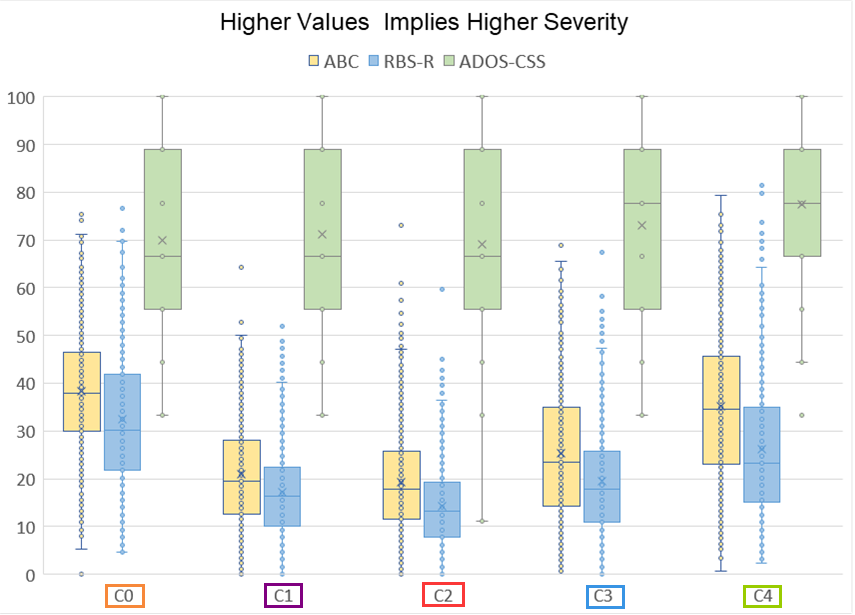
\includegraphics[width=4in]{Higher_Higher.png}
\label{fig:high-highsum}
 }\hspace{2em}\\
\subfigure[\textbf{Outcome Measures for which values are inversely correlated with ASD severity.}]
    {
        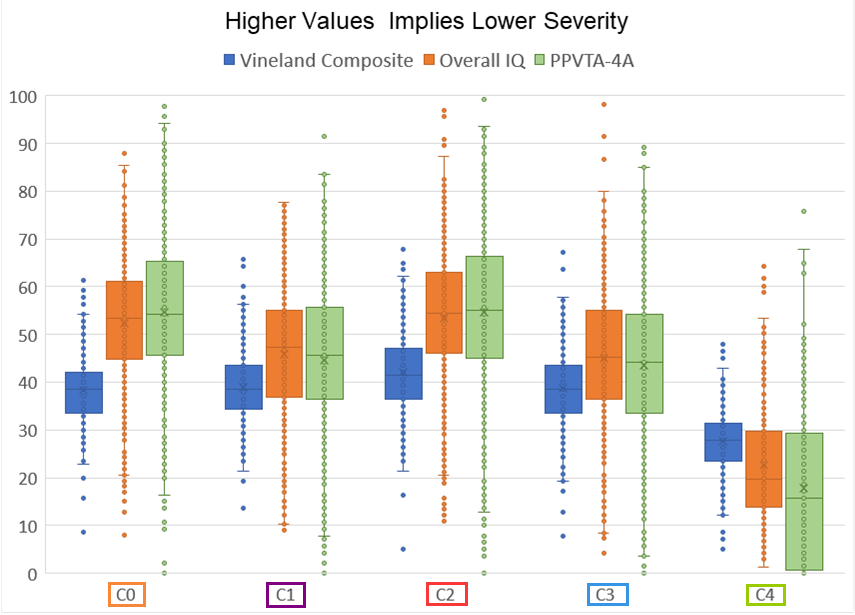
\includegraphics[width=4in]{Higher_lower.png}
        \label{fig:high-lowsum}
    }
    \caption[]{Analysis of ASD outcome measures (normalized values using known features ranges) across clusters for kNN2 Tenacity 5 clustering configuration. The color of the boxes correlate to the colors of the clusters in Figure~\ref{fig:PictureTen2-5}. Gold denotes C0, Purple: C1, Red: C2, Blue: C3, and Green: C4.}
    \label{fig:summ5cluster}
\end{figure}
%\textbf{
%Four of the seven optimal clusterings consisted of 5 clusters.  Two of the clusterings were obtained using integrity (both with and without reassigment) and two of the clusterings were obtained using tenacity (again both with and without reassignment). For both the $k=5$ results shown in Table \ref{tab:autismTableWithNR}, there is a least-affected cluster, cluster C2.  This cluster scores lowest for ABC, RBS-R, and ADOS CSS, and highest for Vineland, IQ and PPVTA 4A.  Interestingly, these clusters have only the second and third lowest incidences of epilepsy.  For both of these clusterings, there is not a consistently most-affected cluster.  For Vineland, IQ and PPVTA, cluster C4 in the Tenacity clustering and cluster C1 in the Integrity clustering are the most affected.  However, for ABC and RBS the highest scores are for cluster C0 in both cases, and for ADOS The highest scores are for cluster C4. 
%The $\eta^2$ values for these clusterings are high across all outcome measures, although they are higher for the kNN 2 Tenacity k=5 clustering.
%The Tenacity k=5 results in Table \ref{tab:autismTableWithNR} correspond to the Tenacity results without reassignment in Table \ref{tab:autismTableWithoutNR}.  Notice that the no-reassignment cluster C1 corresponds to with-reassignment cluster C2 in having the best scores across 6 measures. Interestingly, lack of reassignment did not necessarily result in cleaner clusters.  Half of the measures were better even with reassignment.  The most affected group is split, with C3 scoring worst on the first 3 measures and C2 scoring worst on the last 3.  
%}  

%\textbf{
%The no-reassignment integrity k=5 clustering is unique in that it does not have an unambiguously least-affected cluster.  Cluster C3 scores best on the ABC and RBS-R attributes, while cluster C0 scores best on the other 4 attributes. As with the other 5-clusterings, the most affected group is split, with C1 most affected on ABC and RBS-R and C4 most affected on the other measures. 
%}
 

%The cleanliness of clusters applies to the highest performing group as well.  Without node reassignment, C1 with 951 members has the highest ranking in all measures.  With reassignment, C2 with 781 members has the highest ranking in all measures except epilepsy.  Comparing the two, C2 without node reassignment scores better on all measures except ABC Overall and Stereotyped Behavior (RBS R), and on Vineland Composite Score where scores are approximately the same. Interestingly, variances are higher for the first three features without node reassignment and higher for the last three features with node reassignment.   




%In previous work \cite{ICDM}, kNN graphs at minimum connectivity have tended to yield the most accurate results for datasets with ground truth.  However, the exact setting of the connectivity threshold for the optimal graph representation in this scenario is an open question.  The results indicate that sometimes setting the k threshold above connectivity may yield better clustering as measured via some validation indices.  Out of the top six results, five of them are VAT, suggesting that VAT could possibly outperform Integrity as a node resilience clustering measure. 

%We have shown in previous work \cite{ICDM} that NBR-clust is particularly suited for identification and removal of noise or outliers. We have not considered this scenario in the current work. Our method may be sensitive to the presences of noise. For example, the kNN2VAT (Range) k=5 has a cluster consisting of only 3 nodes.  As shown in Figure \ref{fig:PictureC}, these nodes (yellow) are completely disconnected from the network. Possible removal of those nodes and subsequent reclustering may result in a more optimal configuration.



The feature extraction results seem to suggest that the following phenotypes could be useful biomarkers in delineating ASD subgroups: Regression, Word Delay, ADI-R Q30 (Overall Level of Language), ADI-R Q86 (Abnormality evidence), RBS-R aggregate score (Ritualistic Behavior), ABC aggregate scores (Irritability, Inappropriate Speech), CBCL Externalizing T Score, Verbal score (ADI-R B), RBS-R-Stereotyped Behavior, BAPQ Avg (Mother), ADI-R C (Repetitive Behavior), Social (ADI-R A), and SRS aggregate scores (Mannerisms, Cognition, overall T Score). These results support evidence that language delay, regression and social scores are useful biomarkers for delineating meaningful subgroups. 




\section*{Conclusion}
%The results presented in this paper are the first attempt of applying node-resilience clustering to a biomedical dataset without existing ground truths. The results obtained demonstrate the potential and usefulness of VAT-clust. We plan to further investigate the open questions raised in this work in future analysis.
This paper investigated the application of the NBR-Clust graph-based method to cluster analysis of ASD phenotypes of 2680 simplex ASD probands using different node resilience measures. To determine the optimal clustering configuration, we applied a holistic approach using three main criteria: internal cluster validation indices, graph quality measures, and distribution of
resulting clusters. We presented a rigorous
clinical/behavioral analysis of the highly ranked results by graph type and resilience measure.
The results obtained demonstrate the potential and usefulness of NBR-Clust.
The results favored a 5-cluster ASD sub-grouping configuration and identified a set of potentially useful phenotype biomarkers. Future work will include refinement of the critical attack set to identify specifically the outlier nodes for enhanced biomarker detection. Further studies are also needed to verify the potential ASD biomarkers identified in this work with respect to their application in management of ASD.

%%%%%%%%%%%%%%%%%%%%%%%%%%%%%%%%%%%%%%%%%%%%%%
%%                                          %%
%% Backmatter begins here                   %%
%%                                          %%
%%%%%%%%%%%%%%%%%%%%%%%%%%%%%%%%%%%%%%%%%%%%%%

\begin{backmatter}
\section*{Availability of data and materials}
The data utilized in this work was obtained from the Simons Simplex Collection, supported by Simons Foundation for Autism Research Initiatives (SFARI): www.sfari.org. The data is available upon request by contacting SFARI base directly.  

\section*{Competing interests}
  The authors declare that they have no competing interests.


\section*{No Funding}
  

\section*{Author's contributions}
JM ran all NBR experiments, 
interpreted results of analyses, prepared manuscript figures, contributed to
the conception and design of the study and is the first author of the
manuscript. JZ ran the correlation filter algorithm, cluster validation experiments, conducted the statistical analysis, and prepared the tables for the manuscript. GE supervised all the NBR experiments and guided the interpretation of the analysis, contributed to the conception and design of the study, and participated in drafting and
revising the manuscript. TOA collected the behavioral and clinical data, supervised analyses of these data, contributed to the conception and design of the study, contributed to drafting and revising the manuscript, and is the corresponding author. All authors read and approved the
final manuscript.

\section*{Acknowledgements}
  We appreciate obtaining access to Simons Simplex Collection phenotype data analyzed in this study via SFARI base: www.sfari.org. We also appreciate the support of Ms. Cynthia Germeroth in uploading the data into the SAP HANA in-memory database.
%%%%%%%%%%%%%%%%%%%%%%%%%%%%%%%%%%%%%%%%%%%%%%%%%%%%%%%%%%%%%
%%                  The Bibliography                       %%
%%                                                         %%
%%  Bmc_mathpys.bst  will be used to                       %%
%%  create a .BBL file for submission.                     %%
%%  After submission of the .TEX file,                     %%
%%  you will be prompted to submit your .BBL file.         %%
%%                                                         %%
%%                                                         %%
%%  Note that the displayed Bibliography will not          %%
%%  necessarily be rendered by Latex exactly as specified  %%
%%  in the online Instructions for Authors.                %%
%%                                                         %%
%%%%%%%%%%%%%%%%%%%%%%%%%%%%%%%%%%%%%%%%%%%%%%%%%%%%%%%%%%%%%

% if your bibliography is in bibtex format, use those commands:
\bibliographystyle{bmc-mathphys} % Style BST file (bmc-mathphys, vancouver, spbasic).
\bibliography{bmc_article}      % Bibliography file (usually '*.bib' )
% for author-year bibliography (bmc-mathphys or spbasic)
% a) write to bib file (bmc-mathphys only)
% @settings{label, options="nameyear"}
% b) uncomment next line
%\nocite{label}

% or include bibliography directly:
% \begin{thebibliography}
% \bibitem{b1}
% \end{thebibliography}

%%%%%%%%%%%%%%%%%%%%%%%%%%%%%%%%%%%
%%                               %%
%% Figures                       %%
%%                               %%
%% NB: this is for captions and  %%
%% Titles. All graphics must be  %%
%% submitted separately and NOT  %%
%% included in the Tex document  %%
%%                               %%
%%%%%%%%%%%%%%%%%%%%%%%%%%%%%%%%%%%

%%
%% Do not use \listoffigures as most will included as separate files


%%%%%%%%%%%%%%%%%%%%%%%%%%%%%%%%%%%
%%                               %%
%% Tables                        %%
%%                               %%
%%%%%%%%%%%%%%%%%%%%%%%%%%%%%%%%%%%

%% Use of \listoftables is discouraged.
%%


%%%%%%%%%%%%%%%%%%%%%%%%%%%%%%%%%%%
%%                               %%
%% Additional Files              %%
%%                               %%
%%%%%%%%%%%%%%%%%%%%%%%%%%%%%%%%%%%

%\section*{Additional Files}
%  \subsection*{Additional file 1 --- Sample additional file title}
 %   Additional file descriptions text (including details of how to
 %   view the file, if it is in a non-standard format or the file extension).  This might
 %   refer to a multi-page table or a figure.

 % \subsection*{Additional file 2 --- Sample additional file title}
 %   Additional file descriptions text.


\end{backmatter}
\end{document}
